\documentclass[12pt,a4paper]{article}
\usepackage{hyperref}

\title{Satellite image processing application to the shrinking Aral Sea} 
\author{Alsayed M., Balducci S., Berselli G., Gargiulo F., Rondini T.}
\date{10/01/2023}

\usepackage{amsmath}
\usepackage{amsfonts}
\usepackage{amssymb}
\usepackage{amsthm}
\usepackage{braket}
\usepackage[margin=3cm]{geometry}
\usepackage{pgfplots}
\pgfplotsset{compat=1.18}
\usepackage{fancyhdr}
\usepackage{physics}
\usepackage{systeme,mathtools}
\usepackage{graphicx}
\usepackage{float}
\usepackage{relsize}
\usepackage{calligra}
\usepackage{siunitx}
\usepackage[miktex]{gnuplottex}
\usepackage{epstopdf}
\usepackage[english]{babel}
\usepackage{csquotes}
\usepackage{float}
\floatplacement{figure}{H}
\usepackage{tikz}
\usetikzlibrary{shapes.misc}
\usepackage[style=ieee]{biblatex}
\addbibresource{biblio.bib}
\usepackage{pgf}
\usepackage{caption}
\usepackage{subcaption}

\newcommand{\R}{\Re}
\newcommand{\la}{\lambda}
\newcommand{\al}{\alpha}
\newcommand{\bd}{\textbf}
\newcommand{\rita}{\longrightarrow}
\newcommand{\lang}{\left\langle}
\newcommand{\rang}{\right\rangle}
\newcommand{\lbra}{\left\lbrace}
\newcommand{\rbra}{\right\rbrace}

\begin{document}

\maketitle
\begin{center}
	\url{https://github.com/Grufoony/Aral_Sea_shrinking}
\end{center}

\begin{abstract}
    The aim of this project is to apply image processing techniques to satellite images in order to study a real-life phenomenon, the shrinking of the Aral Sea.
    By applying the basis of image segmentation, we were able to quantify the shrinking ratio through time, thus obtaining a plot of its evolution through a 44-years timespan.
    Moreover, by combining the edge detection technique with operations between more images we were also able to improve the visualization of this phenomenon through an animated GIF.
\end{abstract}
\thispagestyle{empty}

\newpage
\thispagestyle{empty}
\addtocounter{page}{-2}
\mbox{}

\tableofcontents
\pagebreak

\section*{Introduction}
Satellite images are an excellent tool to study landscape’s time evolution both in the long and in the short term and they are freely available in the public domain. 
These are helpful for a wide range of analysis related to human or natural impact on the landscape evolution through time such as urban growth, deforestation, flooding, ice melting, lake shrinking and more. 

In this work we applied image processing’s techniques to multi-temporal satellite images to study the multiannual change of the surface extension of Aral Sea, that was a lake lying between Kazakhstan and the north of Uzbekistan. 
We took the cue from the paper of Vanjare et al. \cite{satelliteImg} in which urban growth of Bangalore region has been studied and discussed by using multi-temporal and multi-spectral Landsat satellite images. 
The aim of this work is to quantify the superficial extension of Aral Sea and its reduction through time due to human activities. We used data from a public archive of the USGS. 
The images are cloudless and of the same resolution, already geo-localized with well-defined coordinates. 
Our analysis is based on simple image processing’s techniques, i.e. image segmentation with a k-mean clustering, thresholding and edge detection.   

The Aral Sea was an endorheic lake lying between Kazakhstan in the north and Uzbekistan in the south which began shrinking in the 1960s and had largely dried up by the 2010s. 
It was formerly the fourth largest lake in the world with a surface area of $68000\,km^2$.  
However, an attempt to grow cottons, melons, rice and cereals in the desert, the so-called Soviet irrigation project, foresaw the deviation of its fed rivers by 1960s. 
From then surface evaporation and lack of rain made the shrinking process rapid. Several attempts were made through time in order to restore the original sea. For example, in $2005$ was completed the building of a dike to prevent the surface extension and the volume of the water in the north basin of the lake, the one lying in Kazakhstan. 
In fact, this side of the lake has nowadays almost the same surface extension than before. 
Unfortunately, the attempts made were not enough: satellite images acquired by NASA in August $2014$ revealed that for the first time in modern history the eastern basin of the Aral Sea had completely dried up. 

\pagebreak

\section{Applied Method}
The general technique to satellite image processing presents some difficulties with acquired images, so, in order to proceed with it, several steps has been made in order to correct our images and  make them suitable for our purpose.  

Acquired images can be generated by different satellites or different lenses and they could have a wide range of extension and resolution. 
We need many images to cover a long-time interval, which may be very different among themselves, so we need to preprocess them in order to overcome those problems. 

The first step is to convert all images in the way they have all the same resolution, with a fixed tolerance. 
In our case we chose photos from a dataset were already re-sampled. 

We must be sure that all images describe the same geographic area. This is essential to compare them, but also to overlap them for both qualitative and quantitative analysis. 
In the study of a big area, it’s common to have also geometric distortion. We have used images already geolocalized which are referred to the same area. 
Landsat’s dataset has a defined path/row extension. Row refers to the latitudinal center line of a frame of imagery. As the satellite moves along its path, the observatory instruments are continuously scanning the terrain below. 
We can convert the path/row of the satellite to a value of lat/long coordinates.  

Our analyzed images were taken from a dataset and for our analysis geometric distortion is not important. 

In order to remove clouds, the general technique concerns to blend multi-spectral images and use a reference no-cloudy image. 
Some algorithms can be improved to distinguish clouds from Earth’s surface. Our images were already cloudless since the Aral Sea is situated in a desert area and clouds are particularly rare in its place. 

For some research issues, we need multi-spectral images \cite{satelliteImg}: sometimes using different material reflectance is the only way to segmentate different objects. For our purposes, it wasn’t essential to use multi-spectral images because the differences between the lake and the surrounding area were evident in terms of both colors and grey levels, so for this work we just used true color images.  

\pagebreak

\section{Surface analysis}
We found images of Aral Sea in the USGS's archive~\cite{images} of different years: $1977$, $1987$, $1998$, $2006$, $2010$, $2013$, $2014$, $2015$, $2019$, $2021$.
They cover a 44-years timespan from the beginning of exploitation of rivers water to our days. 
USGS selects pictures of the same territory (same coordinates reference) so we did not need to geo-localize them. 
The images are $1000 \times 991$ resolution RGB pictures with $32$ bits depth. 
The contrast between water and all other elements is high and there are no clouds; the only similar brightness is the green spots due to vegetation near rivers.

To distinguish water pixels from all the others we used a segmentation technique, the k-mean Clustering of the program ImageJ. 
k-means Clustering is implemented in ImageJ by a plugin~\cite{plugin} and performs a pixel-based segmentation of multi-band images. 
Each pixel in the input image is assigned to one of the clusters. 
Values in the output image produced by the plugin represent cluster number to which original pixel was assigned. 
Each cluster is defined by its centroid in n-dimensional space. 
Pixels are grouped by their proximity to cluster's centroids. 
Cluster centroids are determined using a heuristic: initially centroids are initialized using the k-means algorithm~\cite{kmeans} and then their location is interactively optimized~\cite{plugin}.
We used two or three clusters to optimize segmentation. 
In fact, the segmentation works great with dark (deep) water, but not with light (shallow) one: when the contrast is low is better to use more clusters with respect to the high contrast case. 
Furthermore, the green spots near rivers are classified in the same cluster as the water. 
This is not a problem for two reasons: firstly, the vegetation covers a much smaller area than the water and, secondly, we are interested in the shrinking ratio of the lake and the vegetation disappeared similarly to the water. 
The output of the plugin is a gray level image, as we can see in Fig. \ref{fig:plugin}.
\begin{figure}[H]
    \centering
    \begin{subfigure}[b]{.45\textwidth}
        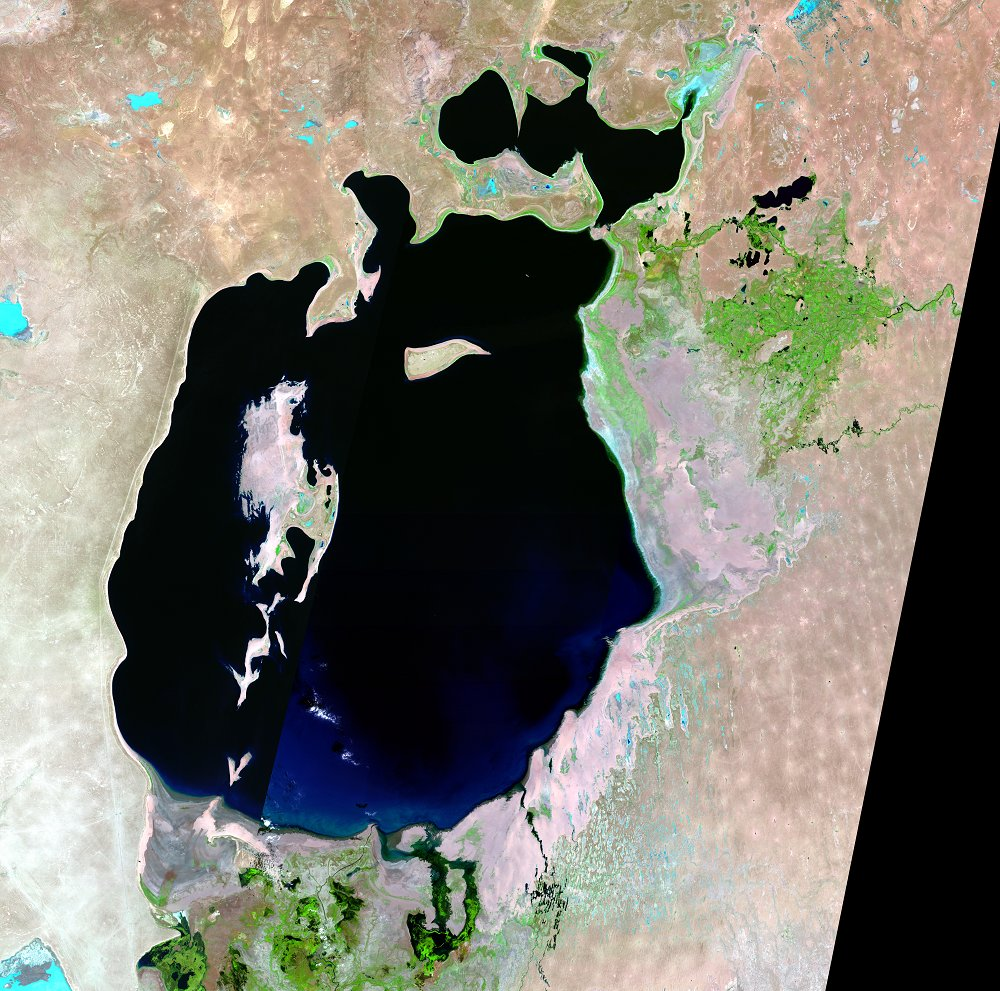
\includegraphics[width=\textwidth]{../img/1987.jpg}
        \caption{\emph{Original image.}}
    \end{subfigure}
    \begin{subfigure}[b]{.45\textwidth}
        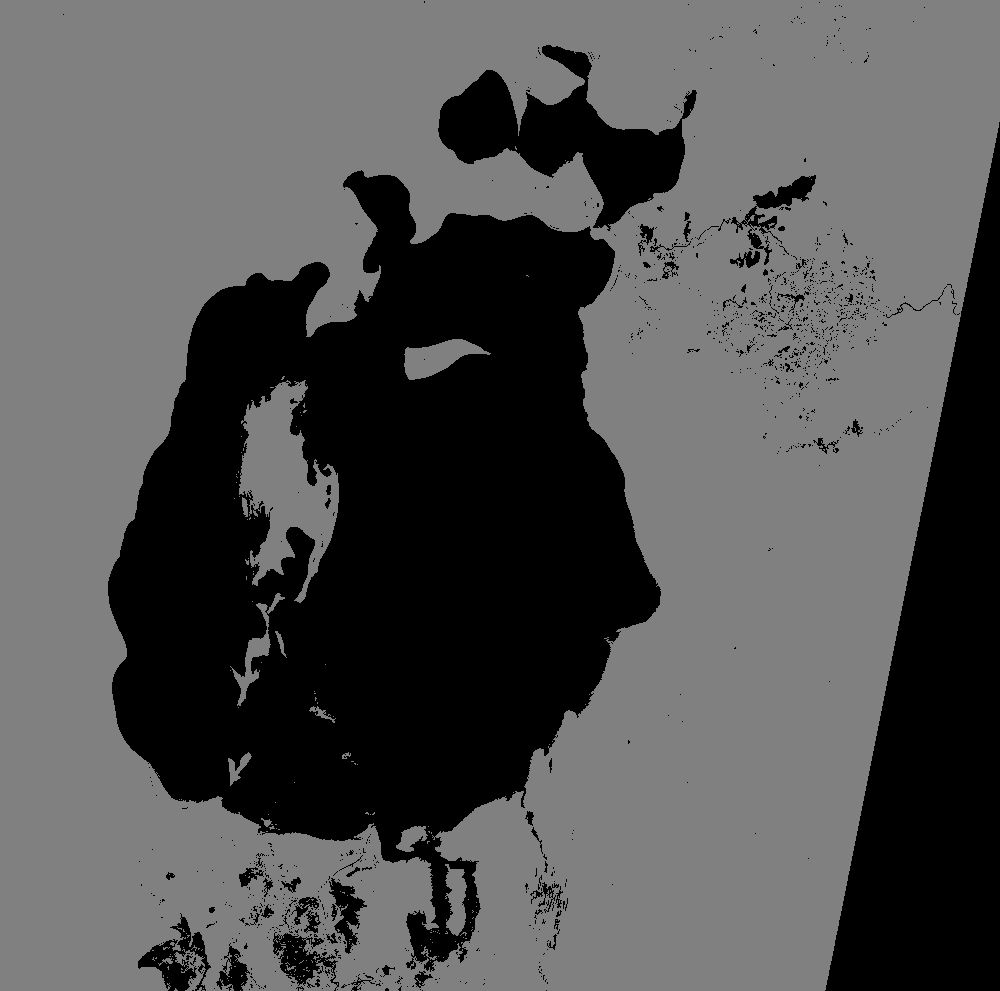
\includegraphics[width=\textwidth]{../img/2clusters.jpg}
        \caption{\emph{Result of k-means clustering.}}
    \end{subfigure}
    \caption{\emph{K-clustering implementation with $k=2$ clusters.}}
    \label{fig:plugin}
\end{figure}
Once obtained the clusters image, using a threshold, we converted the images in binary ones: in this way we were able to separate the object (the sea) from the background, and count how many pixels represent water. 
At this point, to compute the areal ratio, it is sufficient to divide the number of water pixels by a reference value. 
We set this value to be the water surface of $1977$, i.e. the maximal extension of the lake. 
Furthermore, we use the image from $1977$ as a mask for the others: in this way we can filter the lake's water pixels by considering as lake only the pixels that were water in $1977$.
The result consist in a well constructed filter, as we can see in Fig. \ref{fig:masking}.
\begin{figure}[H]
    \centering
    \begin{subfigure}[b]{.45\textwidth}
        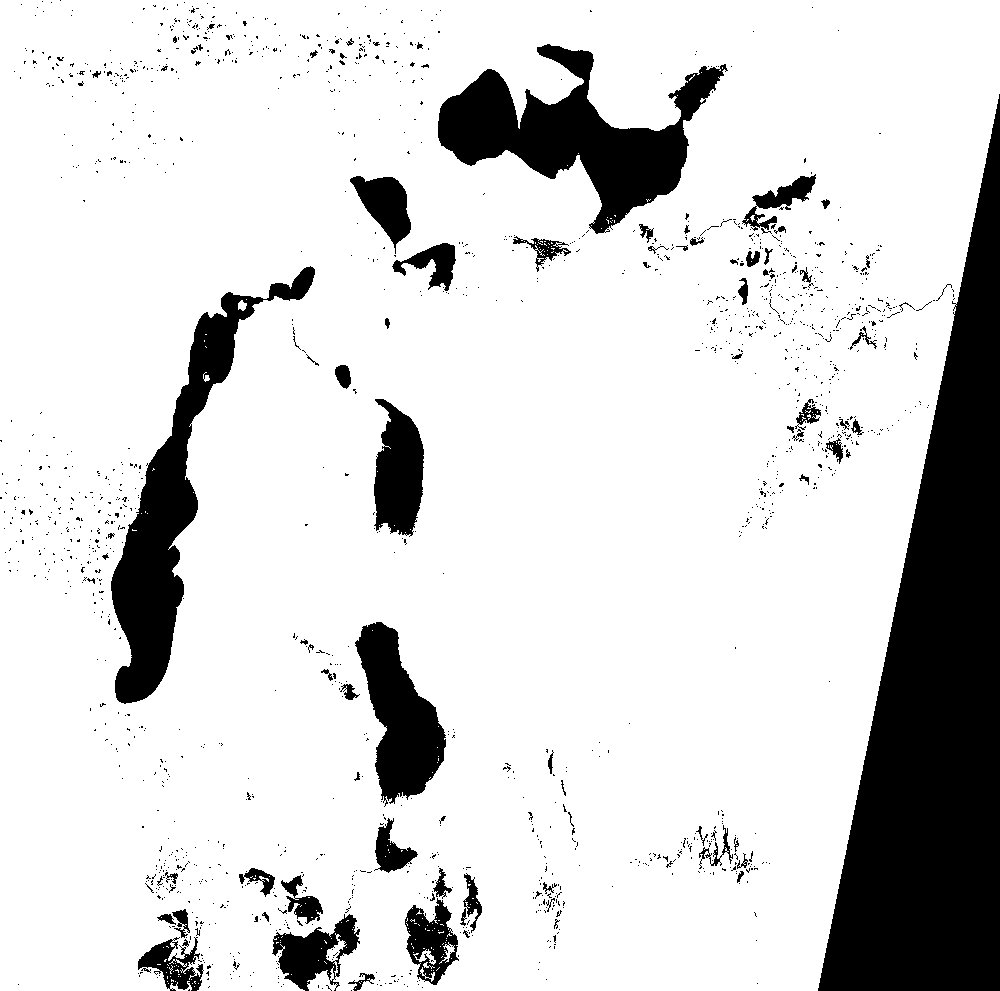
\includegraphics[width=\textwidth]{../img/2015_with_noise.jpg}
        \caption{\emph{Thresholded k-means clustering's output.}}
    \end{subfigure}
    \begin{subfigure}[b]{.45\textwidth}
        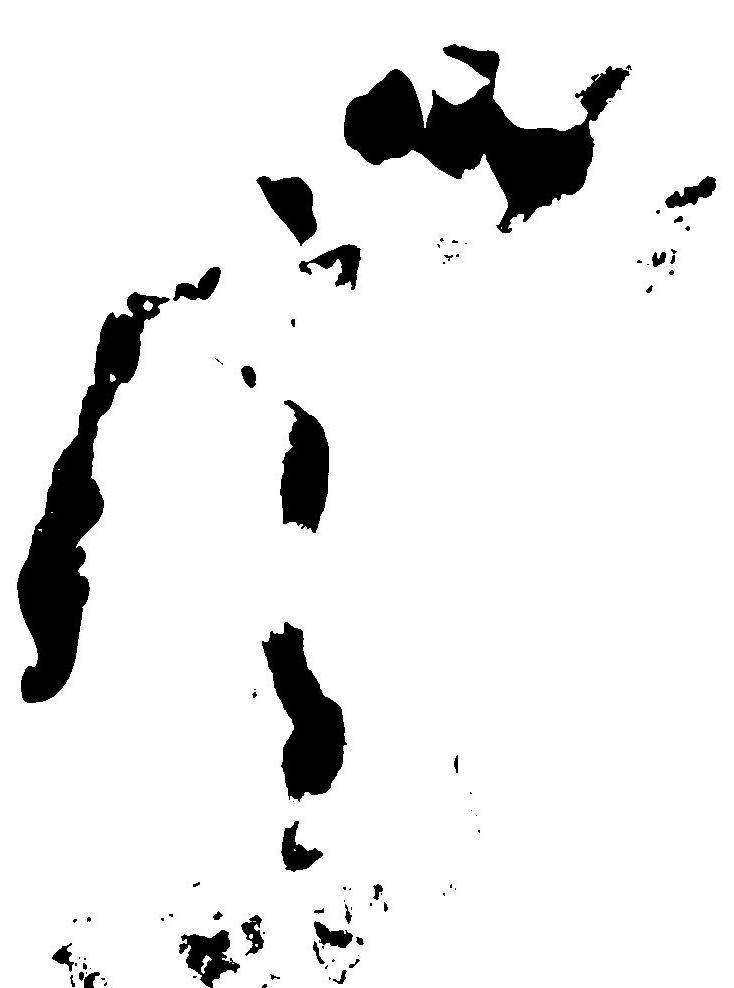
\includegraphics[width=\textwidth]{../img/2015w.jpg}
        \caption{\emph{Masking result with image \\from 1977.}}
    \end{subfigure}
    \caption{\emph{Comparison between unmasked (a) and masked (b) threshold.}}
    \label{fig:masking}
\end{figure}
To remove isolated pixels classified as sea's water we applied a median filter implemented in ImageJ, the ``despeckle'' filter. 
This is a median filter that replaces each pixel with the median value in its $3 \times 3$ neighborhood~\cite{despeckle}.
We removed these points because they represent a residual noise from the previous steps (k-mean clustering and threshold): they are dark points in the background. 
This filter allows a better visualization of the images, and their area is negligible respect the total.

The result of the analysis is reported in appendix. 
Once we isolated water pixels in all the images, we were able to plot the evolution of shrinking ratio through time. 
We can see that the total surface area of the lake is decreasing with an almost linear trend. 
In fact, although there were attempts to preserve the north side of the lake with good results, the other side of it, the one with the majority of surface extension, was totally abandoned after the soviet irrigation project. 
We don't have enough data to explain a linear decreasing with time of the Aral Sea's surface area, but we can say that, after the deviation of its fed rivers, the water volume total balance was regulated by surface evaporation and total precipitation in the area. 
This balance is a part of the water cycle, and it is almost constant during a year cycle, even if the evaporation rate is slowly increasing because of global warming. 
Of course, in a desert area as the one we have analyzed, we expect that evaporation dominates over precipitation resulting in an almost constant surface area decrease through time.
In Fig. \ref{fig:expo} we can see this linear trend.
\begin{figure}[H]
    \centering
    \scalebox{.7}{%% Creator: Matplotlib, PGF backend
%%
%% To include the figure in your LaTeX document, write
%%   \input{<filename>.pgf}
%%
%% Make sure the required packages are loaded in your preamble
%%   \usepackage{pgf}
%%
%% Also ensure that all the required font packages are loaded; for instance,
%% the lmodern package is sometimes necessary when using math font.
%%   \usepackage{lmodern}
%%
%% Figures using additional raster images can only be included by \input if
%% they are in the same directory as the main LaTeX file. For loading figures
%% from other directories you can use the `import` package
%%   \usepackage{import}
%%
%% and then include the figures with
%%   \import{<path to file>}{<filename>.pgf}
%%
%% Matplotlib used the following preamble
%%   \usepackage{fontspec}
%%   \setmainfont{DejaVuSerif.ttf}[Path=\detokenize{/home/simone/.local/lib/python3.10/site-packages/matplotlib/mpl-data/fonts/ttf/}]
%%   \setsansfont{DejaVuSans.ttf}[Path=\detokenize{/home/simone/.local/lib/python3.10/site-packages/matplotlib/mpl-data/fonts/ttf/}]
%%   \setmonofont{DejaVuSansMono.ttf}[Path=\detokenize{/home/simone/.local/lib/python3.10/site-packages/matplotlib/mpl-data/fonts/ttf/}]
%%
\begingroup%
\makeatletter%
\begin{pgfpicture}%
\pgfpathrectangle{\pgfpointorigin}{\pgfqpoint{6.400000in}{4.800000in}}%
\pgfusepath{use as bounding box, clip}%
\begin{pgfscope}%
\pgfsetbuttcap%
\pgfsetmiterjoin%
\definecolor{currentfill}{rgb}{1.000000,1.000000,1.000000}%
\pgfsetfillcolor{currentfill}%
\pgfsetlinewidth{0.000000pt}%
\definecolor{currentstroke}{rgb}{1.000000,1.000000,1.000000}%
\pgfsetstrokecolor{currentstroke}%
\pgfsetdash{}{0pt}%
\pgfpathmoveto{\pgfqpoint{0.000000in}{0.000000in}}%
\pgfpathlineto{\pgfqpoint{6.400000in}{0.000000in}}%
\pgfpathlineto{\pgfqpoint{6.400000in}{4.800000in}}%
\pgfpathlineto{\pgfqpoint{0.000000in}{4.800000in}}%
\pgfpathlineto{\pgfqpoint{0.000000in}{0.000000in}}%
\pgfpathclose%
\pgfusepath{fill}%
\end{pgfscope}%
\begin{pgfscope}%
\pgfsetbuttcap%
\pgfsetmiterjoin%
\definecolor{currentfill}{rgb}{1.000000,1.000000,1.000000}%
\pgfsetfillcolor{currentfill}%
\pgfsetlinewidth{0.000000pt}%
\definecolor{currentstroke}{rgb}{0.000000,0.000000,0.000000}%
\pgfsetstrokecolor{currentstroke}%
\pgfsetstrokeopacity{0.000000}%
\pgfsetdash{}{0pt}%
\pgfpathmoveto{\pgfqpoint{0.800000in}{0.528000in}}%
\pgfpathlineto{\pgfqpoint{5.760000in}{0.528000in}}%
\pgfpathlineto{\pgfqpoint{5.760000in}{4.224000in}}%
\pgfpathlineto{\pgfqpoint{0.800000in}{4.224000in}}%
\pgfpathlineto{\pgfqpoint{0.800000in}{0.528000in}}%
\pgfpathclose%
\pgfusepath{fill}%
\end{pgfscope}%
\begin{pgfscope}%
\pgfsetbuttcap%
\pgfsetroundjoin%
\definecolor{currentfill}{rgb}{0.000000,0.000000,0.000000}%
\pgfsetfillcolor{currentfill}%
\pgfsetlinewidth{0.803000pt}%
\definecolor{currentstroke}{rgb}{0.000000,0.000000,0.000000}%
\pgfsetstrokecolor{currentstroke}%
\pgfsetdash{}{0pt}%
\pgfsys@defobject{currentmarker}{\pgfqpoint{0.000000in}{-0.048611in}}{\pgfqpoint{0.000000in}{0.000000in}}{%
\pgfpathmoveto{\pgfqpoint{0.000000in}{0.000000in}}%
\pgfpathlineto{\pgfqpoint{0.000000in}{-0.048611in}}%
\pgfusepath{stroke,fill}%
}%
\begin{pgfscope}%
\pgfsys@transformshift{1.332893in}{0.528000in}%
\pgfsys@useobject{currentmarker}{}%
\end{pgfscope}%
\end{pgfscope}%
\begin{pgfscope}%
\definecolor{textcolor}{rgb}{0.000000,0.000000,0.000000}%
\pgfsetstrokecolor{textcolor}%
\pgfsetfillcolor{textcolor}%
\pgftext[x=1.332893in,y=0.430778in,,top]{\color{textcolor}\sffamily\fontsize{15.000000}{18.000000}\selectfont 1980}%
\end{pgfscope}%
\begin{pgfscope}%
\pgfsetbuttcap%
\pgfsetroundjoin%
\definecolor{currentfill}{rgb}{0.000000,0.000000,0.000000}%
\pgfsetfillcolor{currentfill}%
\pgfsetlinewidth{0.803000pt}%
\definecolor{currentstroke}{rgb}{0.000000,0.000000,0.000000}%
\pgfsetstrokecolor{currentstroke}%
\pgfsetdash{}{0pt}%
\pgfsys@defobject{currentmarker}{\pgfqpoint{0.000000in}{-0.048611in}}{\pgfqpoint{0.000000in}{0.000000in}}{%
\pgfpathmoveto{\pgfqpoint{0.000000in}{0.000000in}}%
\pgfpathlineto{\pgfqpoint{0.000000in}{-0.048611in}}%
\pgfusepath{stroke,fill}%
}%
\begin{pgfscope}%
\pgfsys@transformshift{2.357686in}{0.528000in}%
\pgfsys@useobject{currentmarker}{}%
\end{pgfscope}%
\end{pgfscope}%
\begin{pgfscope}%
\definecolor{textcolor}{rgb}{0.000000,0.000000,0.000000}%
\pgfsetstrokecolor{textcolor}%
\pgfsetfillcolor{textcolor}%
\pgftext[x=2.357686in,y=0.430778in,,top]{\color{textcolor}\sffamily\fontsize{15.000000}{18.000000}\selectfont 1990}%
\end{pgfscope}%
\begin{pgfscope}%
\pgfsetbuttcap%
\pgfsetroundjoin%
\definecolor{currentfill}{rgb}{0.000000,0.000000,0.000000}%
\pgfsetfillcolor{currentfill}%
\pgfsetlinewidth{0.803000pt}%
\definecolor{currentstroke}{rgb}{0.000000,0.000000,0.000000}%
\pgfsetstrokecolor{currentstroke}%
\pgfsetdash{}{0pt}%
\pgfsys@defobject{currentmarker}{\pgfqpoint{0.000000in}{-0.048611in}}{\pgfqpoint{0.000000in}{0.000000in}}{%
\pgfpathmoveto{\pgfqpoint{0.000000in}{0.000000in}}%
\pgfpathlineto{\pgfqpoint{0.000000in}{-0.048611in}}%
\pgfusepath{stroke,fill}%
}%
\begin{pgfscope}%
\pgfsys@transformshift{3.382479in}{0.528000in}%
\pgfsys@useobject{currentmarker}{}%
\end{pgfscope}%
\end{pgfscope}%
\begin{pgfscope}%
\definecolor{textcolor}{rgb}{0.000000,0.000000,0.000000}%
\pgfsetstrokecolor{textcolor}%
\pgfsetfillcolor{textcolor}%
\pgftext[x=3.382479in,y=0.430778in,,top]{\color{textcolor}\sffamily\fontsize{15.000000}{18.000000}\selectfont 2000}%
\end{pgfscope}%
\begin{pgfscope}%
\pgfsetbuttcap%
\pgfsetroundjoin%
\definecolor{currentfill}{rgb}{0.000000,0.000000,0.000000}%
\pgfsetfillcolor{currentfill}%
\pgfsetlinewidth{0.803000pt}%
\definecolor{currentstroke}{rgb}{0.000000,0.000000,0.000000}%
\pgfsetstrokecolor{currentstroke}%
\pgfsetdash{}{0pt}%
\pgfsys@defobject{currentmarker}{\pgfqpoint{0.000000in}{-0.048611in}}{\pgfqpoint{0.000000in}{0.000000in}}{%
\pgfpathmoveto{\pgfqpoint{0.000000in}{0.000000in}}%
\pgfpathlineto{\pgfqpoint{0.000000in}{-0.048611in}}%
\pgfusepath{stroke,fill}%
}%
\begin{pgfscope}%
\pgfsys@transformshift{4.407273in}{0.528000in}%
\pgfsys@useobject{currentmarker}{}%
\end{pgfscope}%
\end{pgfscope}%
\begin{pgfscope}%
\definecolor{textcolor}{rgb}{0.000000,0.000000,0.000000}%
\pgfsetstrokecolor{textcolor}%
\pgfsetfillcolor{textcolor}%
\pgftext[x=4.407273in,y=0.430778in,,top]{\color{textcolor}\sffamily\fontsize{15.000000}{18.000000}\selectfont 2010}%
\end{pgfscope}%
\begin{pgfscope}%
\pgfsetbuttcap%
\pgfsetroundjoin%
\definecolor{currentfill}{rgb}{0.000000,0.000000,0.000000}%
\pgfsetfillcolor{currentfill}%
\pgfsetlinewidth{0.803000pt}%
\definecolor{currentstroke}{rgb}{0.000000,0.000000,0.000000}%
\pgfsetstrokecolor{currentstroke}%
\pgfsetdash{}{0pt}%
\pgfsys@defobject{currentmarker}{\pgfqpoint{0.000000in}{-0.048611in}}{\pgfqpoint{0.000000in}{0.000000in}}{%
\pgfpathmoveto{\pgfqpoint{0.000000in}{0.000000in}}%
\pgfpathlineto{\pgfqpoint{0.000000in}{-0.048611in}}%
\pgfusepath{stroke,fill}%
}%
\begin{pgfscope}%
\pgfsys@transformshift{5.432066in}{0.528000in}%
\pgfsys@useobject{currentmarker}{}%
\end{pgfscope}%
\end{pgfscope}%
\begin{pgfscope}%
\definecolor{textcolor}{rgb}{0.000000,0.000000,0.000000}%
\pgfsetstrokecolor{textcolor}%
\pgfsetfillcolor{textcolor}%
\pgftext[x=5.432066in,y=0.430778in,,top]{\color{textcolor}\sffamily\fontsize{15.000000}{18.000000}\selectfont 2020}%
\end{pgfscope}%
\begin{pgfscope}%
\definecolor{textcolor}{rgb}{0.000000,0.000000,0.000000}%
\pgfsetstrokecolor{textcolor}%
\pgfsetfillcolor{textcolor}%
\pgftext[x=3.280000in,y=0.173603in,,top]{\color{textcolor}\sffamily\fontsize{15.000000}{18.000000}\selectfont Time (years)}%
\end{pgfscope}%
\begin{pgfscope}%
\pgfsetbuttcap%
\pgfsetroundjoin%
\definecolor{currentfill}{rgb}{0.000000,0.000000,0.000000}%
\pgfsetfillcolor{currentfill}%
\pgfsetlinewidth{0.803000pt}%
\definecolor{currentstroke}{rgb}{0.000000,0.000000,0.000000}%
\pgfsetstrokecolor{currentstroke}%
\pgfsetdash{}{0pt}%
\pgfsys@defobject{currentmarker}{\pgfqpoint{-0.048611in}{0.000000in}}{\pgfqpoint{-0.000000in}{0.000000in}}{%
\pgfpathmoveto{\pgfqpoint{-0.000000in}{0.000000in}}%
\pgfpathlineto{\pgfqpoint{-0.048611in}{0.000000in}}%
\pgfusepath{stroke,fill}%
}%
\begin{pgfscope}%
\pgfsys@transformshift{0.800000in}{0.705248in}%
\pgfsys@useobject{currentmarker}{}%
\end{pgfscope}%
\end{pgfscope}%
\begin{pgfscope}%
\definecolor{textcolor}{rgb}{0.000000,0.000000,0.000000}%
\pgfsetstrokecolor{textcolor}%
\pgfsetfillcolor{textcolor}%
\pgftext[x=0.371459in, y=0.626106in, left, base]{\color{textcolor}\sffamily\fontsize{15.000000}{18.000000}\selectfont 0.0}%
\end{pgfscope}%
\begin{pgfscope}%
\pgfsetbuttcap%
\pgfsetroundjoin%
\definecolor{currentfill}{rgb}{0.000000,0.000000,0.000000}%
\pgfsetfillcolor{currentfill}%
\pgfsetlinewidth{0.803000pt}%
\definecolor{currentstroke}{rgb}{0.000000,0.000000,0.000000}%
\pgfsetstrokecolor{currentstroke}%
\pgfsetdash{}{0pt}%
\pgfsys@defobject{currentmarker}{\pgfqpoint{-0.048611in}{0.000000in}}{\pgfqpoint{-0.000000in}{0.000000in}}{%
\pgfpathmoveto{\pgfqpoint{-0.000000in}{0.000000in}}%
\pgfpathlineto{\pgfqpoint{-0.048611in}{0.000000in}}%
\pgfusepath{stroke,fill}%
}%
\begin{pgfscope}%
\pgfsys@transformshift{0.800000in}{1.375398in}%
\pgfsys@useobject{currentmarker}{}%
\end{pgfscope}%
\end{pgfscope}%
\begin{pgfscope}%
\definecolor{textcolor}{rgb}{0.000000,0.000000,0.000000}%
\pgfsetstrokecolor{textcolor}%
\pgfsetfillcolor{textcolor}%
\pgftext[x=0.371459in, y=1.296256in, left, base]{\color{textcolor}\sffamily\fontsize{15.000000}{18.000000}\selectfont 0.2}%
\end{pgfscope}%
\begin{pgfscope}%
\pgfsetbuttcap%
\pgfsetroundjoin%
\definecolor{currentfill}{rgb}{0.000000,0.000000,0.000000}%
\pgfsetfillcolor{currentfill}%
\pgfsetlinewidth{0.803000pt}%
\definecolor{currentstroke}{rgb}{0.000000,0.000000,0.000000}%
\pgfsetstrokecolor{currentstroke}%
\pgfsetdash{}{0pt}%
\pgfsys@defobject{currentmarker}{\pgfqpoint{-0.048611in}{0.000000in}}{\pgfqpoint{-0.000000in}{0.000000in}}{%
\pgfpathmoveto{\pgfqpoint{-0.000000in}{0.000000in}}%
\pgfpathlineto{\pgfqpoint{-0.048611in}{0.000000in}}%
\pgfusepath{stroke,fill}%
}%
\begin{pgfscope}%
\pgfsys@transformshift{0.800000in}{2.045549in}%
\pgfsys@useobject{currentmarker}{}%
\end{pgfscope}%
\end{pgfscope}%
\begin{pgfscope}%
\definecolor{textcolor}{rgb}{0.000000,0.000000,0.000000}%
\pgfsetstrokecolor{textcolor}%
\pgfsetfillcolor{textcolor}%
\pgftext[x=0.371459in, y=1.966407in, left, base]{\color{textcolor}\sffamily\fontsize{15.000000}{18.000000}\selectfont 0.4}%
\end{pgfscope}%
\begin{pgfscope}%
\pgfsetbuttcap%
\pgfsetroundjoin%
\definecolor{currentfill}{rgb}{0.000000,0.000000,0.000000}%
\pgfsetfillcolor{currentfill}%
\pgfsetlinewidth{0.803000pt}%
\definecolor{currentstroke}{rgb}{0.000000,0.000000,0.000000}%
\pgfsetstrokecolor{currentstroke}%
\pgfsetdash{}{0pt}%
\pgfsys@defobject{currentmarker}{\pgfqpoint{-0.048611in}{0.000000in}}{\pgfqpoint{-0.000000in}{0.000000in}}{%
\pgfpathmoveto{\pgfqpoint{-0.000000in}{0.000000in}}%
\pgfpathlineto{\pgfqpoint{-0.048611in}{0.000000in}}%
\pgfusepath{stroke,fill}%
}%
\begin{pgfscope}%
\pgfsys@transformshift{0.800000in}{2.715699in}%
\pgfsys@useobject{currentmarker}{}%
\end{pgfscope}%
\end{pgfscope}%
\begin{pgfscope}%
\definecolor{textcolor}{rgb}{0.000000,0.000000,0.000000}%
\pgfsetstrokecolor{textcolor}%
\pgfsetfillcolor{textcolor}%
\pgftext[x=0.371459in, y=2.636557in, left, base]{\color{textcolor}\sffamily\fontsize{15.000000}{18.000000}\selectfont 0.6}%
\end{pgfscope}%
\begin{pgfscope}%
\pgfsetbuttcap%
\pgfsetroundjoin%
\definecolor{currentfill}{rgb}{0.000000,0.000000,0.000000}%
\pgfsetfillcolor{currentfill}%
\pgfsetlinewidth{0.803000pt}%
\definecolor{currentstroke}{rgb}{0.000000,0.000000,0.000000}%
\pgfsetstrokecolor{currentstroke}%
\pgfsetdash{}{0pt}%
\pgfsys@defobject{currentmarker}{\pgfqpoint{-0.048611in}{0.000000in}}{\pgfqpoint{-0.000000in}{0.000000in}}{%
\pgfpathmoveto{\pgfqpoint{-0.000000in}{0.000000in}}%
\pgfpathlineto{\pgfqpoint{-0.048611in}{0.000000in}}%
\pgfusepath{stroke,fill}%
}%
\begin{pgfscope}%
\pgfsys@transformshift{0.800000in}{3.385850in}%
\pgfsys@useobject{currentmarker}{}%
\end{pgfscope}%
\end{pgfscope}%
\begin{pgfscope}%
\definecolor{textcolor}{rgb}{0.000000,0.000000,0.000000}%
\pgfsetstrokecolor{textcolor}%
\pgfsetfillcolor{textcolor}%
\pgftext[x=0.371459in, y=3.306707in, left, base]{\color{textcolor}\sffamily\fontsize{15.000000}{18.000000}\selectfont 0.8}%
\end{pgfscope}%
\begin{pgfscope}%
\pgfsetbuttcap%
\pgfsetroundjoin%
\definecolor{currentfill}{rgb}{0.000000,0.000000,0.000000}%
\pgfsetfillcolor{currentfill}%
\pgfsetlinewidth{0.803000pt}%
\definecolor{currentstroke}{rgb}{0.000000,0.000000,0.000000}%
\pgfsetstrokecolor{currentstroke}%
\pgfsetdash{}{0pt}%
\pgfsys@defobject{currentmarker}{\pgfqpoint{-0.048611in}{0.000000in}}{\pgfqpoint{-0.000000in}{0.000000in}}{%
\pgfpathmoveto{\pgfqpoint{-0.000000in}{0.000000in}}%
\pgfpathlineto{\pgfqpoint{-0.048611in}{0.000000in}}%
\pgfusepath{stroke,fill}%
}%
\begin{pgfscope}%
\pgfsys@transformshift{0.800000in}{4.056000in}%
\pgfsys@useobject{currentmarker}{}%
\end{pgfscope}%
\end{pgfscope}%
\begin{pgfscope}%
\definecolor{textcolor}{rgb}{0.000000,0.000000,0.000000}%
\pgfsetstrokecolor{textcolor}%
\pgfsetfillcolor{textcolor}%
\pgftext[x=0.371459in, y=3.976858in, left, base]{\color{textcolor}\sffamily\fontsize{15.000000}{18.000000}\selectfont 1.0}%
\end{pgfscope}%
\begin{pgfscope}%
\definecolor{textcolor}{rgb}{0.000000,0.000000,0.000000}%
\pgfsetstrokecolor{textcolor}%
\pgfsetfillcolor{textcolor}%
\pgftext[x=0.315903in,y=2.376000in,,bottom,rotate=90.000000]{\color{textcolor}\sffamily\fontsize{15.000000}{18.000000}\selectfont Surface ratio}%
\end{pgfscope}%
\begin{pgfscope}%
\pgfpathrectangle{\pgfqpoint{0.800000in}{0.528000in}}{\pgfqpoint{4.960000in}{3.696000in}}%
\pgfusepath{clip}%
\pgfsetrectcap%
\pgfsetroundjoin%
\pgfsetlinewidth{1.505625pt}%
\definecolor{currentstroke}{rgb}{0.121569,0.466667,0.705882}%
\pgfsetstrokecolor{currentstroke}%
\pgfsetdash{}{0pt}%
\pgfpathmoveto{\pgfqpoint{1.025455in}{4.056000in}}%
\pgfpathlineto{\pgfqpoint{2.050248in}{3.296385in}}%
\pgfpathlineto{\pgfqpoint{3.177521in}{2.472100in}}%
\pgfpathlineto{\pgfqpoint{3.997355in}{1.432026in}}%
\pgfpathlineto{\pgfqpoint{4.407273in}{1.394833in}}%
\pgfpathlineto{\pgfqpoint{4.714711in}{1.326477in}}%
\pgfpathlineto{\pgfqpoint{4.817190in}{1.008156in}}%
\pgfpathlineto{\pgfqpoint{4.919669in}{1.182060in}}%
\pgfpathlineto{\pgfqpoint{5.329587in}{0.993078in}}%
\pgfpathlineto{\pgfqpoint{5.534545in}{0.980345in}}%
\pgfusepath{stroke}%
\end{pgfscope}%
\begin{pgfscope}%
\pgfpathrectangle{\pgfqpoint{0.800000in}{0.528000in}}{\pgfqpoint{4.960000in}{3.696000in}}%
\pgfusepath{clip}%
\pgfsetbuttcap%
\pgfsetroundjoin%
\definecolor{currentfill}{rgb}{0.000000,0.000000,1.000000}%
\pgfsetfillcolor{currentfill}%
\pgfsetlinewidth{1.003750pt}%
\definecolor{currentstroke}{rgb}{0.000000,0.000000,1.000000}%
\pgfsetstrokecolor{currentstroke}%
\pgfsetdash{}{0pt}%
\pgfsys@defobject{currentmarker}{\pgfqpoint{-0.041667in}{-0.041667in}}{\pgfqpoint{0.041667in}{0.041667in}}{%
\pgfpathmoveto{\pgfqpoint{0.000000in}{-0.041667in}}%
\pgfpathcurveto{\pgfqpoint{0.011050in}{-0.041667in}}{\pgfqpoint{0.021649in}{-0.037276in}}{\pgfqpoint{0.029463in}{-0.029463in}}%
\pgfpathcurveto{\pgfqpoint{0.037276in}{-0.021649in}}{\pgfqpoint{0.041667in}{-0.011050in}}{\pgfqpoint{0.041667in}{0.000000in}}%
\pgfpathcurveto{\pgfqpoint{0.041667in}{0.011050in}}{\pgfqpoint{0.037276in}{0.021649in}}{\pgfqpoint{0.029463in}{0.029463in}}%
\pgfpathcurveto{\pgfqpoint{0.021649in}{0.037276in}}{\pgfqpoint{0.011050in}{0.041667in}}{\pgfqpoint{0.000000in}{0.041667in}}%
\pgfpathcurveto{\pgfqpoint{-0.011050in}{0.041667in}}{\pgfqpoint{-0.021649in}{0.037276in}}{\pgfqpoint{-0.029463in}{0.029463in}}%
\pgfpathcurveto{\pgfqpoint{-0.037276in}{0.021649in}}{\pgfqpoint{-0.041667in}{0.011050in}}{\pgfqpoint{-0.041667in}{0.000000in}}%
\pgfpathcurveto{\pgfqpoint{-0.041667in}{-0.011050in}}{\pgfqpoint{-0.037276in}{-0.021649in}}{\pgfqpoint{-0.029463in}{-0.029463in}}%
\pgfpathcurveto{\pgfqpoint{-0.021649in}{-0.037276in}}{\pgfqpoint{-0.011050in}{-0.041667in}}{\pgfqpoint{0.000000in}{-0.041667in}}%
\pgfpathlineto{\pgfqpoint{0.000000in}{-0.041667in}}%
\pgfpathclose%
\pgfusepath{stroke,fill}%
}%
\begin{pgfscope}%
\pgfsys@transformshift{1.025455in}{4.056000in}%
\pgfsys@useobject{currentmarker}{}%
\end{pgfscope}%
\begin{pgfscope}%
\pgfsys@transformshift{2.050248in}{3.296385in}%
\pgfsys@useobject{currentmarker}{}%
\end{pgfscope}%
\begin{pgfscope}%
\pgfsys@transformshift{3.177521in}{2.472100in}%
\pgfsys@useobject{currentmarker}{}%
\end{pgfscope}%
\begin{pgfscope}%
\pgfsys@transformshift{3.997355in}{1.432026in}%
\pgfsys@useobject{currentmarker}{}%
\end{pgfscope}%
\begin{pgfscope}%
\pgfsys@transformshift{4.407273in}{1.394833in}%
\pgfsys@useobject{currentmarker}{}%
\end{pgfscope}%
\begin{pgfscope}%
\pgfsys@transformshift{4.714711in}{1.326477in}%
\pgfsys@useobject{currentmarker}{}%
\end{pgfscope}%
\begin{pgfscope}%
\pgfsys@transformshift{4.817190in}{1.008156in}%
\pgfsys@useobject{currentmarker}{}%
\end{pgfscope}%
\begin{pgfscope}%
\pgfsys@transformshift{4.919669in}{1.182060in}%
\pgfsys@useobject{currentmarker}{}%
\end{pgfscope}%
\begin{pgfscope}%
\pgfsys@transformshift{5.329587in}{0.993078in}%
\pgfsys@useobject{currentmarker}{}%
\end{pgfscope}%
\begin{pgfscope}%
\pgfsys@transformshift{5.534545in}{0.980345in}%
\pgfsys@useobject{currentmarker}{}%
\end{pgfscope}%
\end{pgfscope}%
\begin{pgfscope}%
\pgfpathrectangle{\pgfqpoint{0.800000in}{0.528000in}}{\pgfqpoint{4.960000in}{3.696000in}}%
\pgfusepath{clip}%
\pgfsetrectcap%
\pgfsetroundjoin%
\pgfsetlinewidth{1.505625pt}%
\definecolor{currentstroke}{rgb}{1.000000,0.498039,0.054902}%
\pgfsetstrokecolor{currentstroke}%
\pgfsetdash{}{0pt}%
\pgfpathmoveto{\pgfqpoint{1.025455in}{3.963117in}}%
\pgfpathlineto{\pgfqpoint{2.050248in}{3.220591in}}%
\pgfpathlineto{\pgfqpoint{3.177521in}{2.403811in}}%
\pgfpathlineto{\pgfqpoint{3.997355in}{1.809790in}}%
\pgfpathlineto{\pgfqpoint{4.407273in}{1.512779in}}%
\pgfpathlineto{\pgfqpoint{4.714711in}{1.290021in}}%
\pgfpathlineto{\pgfqpoint{4.817190in}{1.215769in}}%
\pgfpathlineto{\pgfqpoint{4.919669in}{1.141516in}}%
\pgfpathlineto{\pgfqpoint{5.329587in}{0.844505in}}%
\pgfpathlineto{\pgfqpoint{5.534545in}{0.696000in}}%
\pgfusepath{stroke}%
\end{pgfscope}%
\begin{pgfscope}%
\pgfsetrectcap%
\pgfsetmiterjoin%
\pgfsetlinewidth{0.803000pt}%
\definecolor{currentstroke}{rgb}{0.000000,0.000000,0.000000}%
\pgfsetstrokecolor{currentstroke}%
\pgfsetdash{}{0pt}%
\pgfpathmoveto{\pgfqpoint{0.800000in}{0.528000in}}%
\pgfpathlineto{\pgfqpoint{0.800000in}{4.224000in}}%
\pgfusepath{stroke}%
\end{pgfscope}%
\begin{pgfscope}%
\pgfsetrectcap%
\pgfsetmiterjoin%
\pgfsetlinewidth{0.803000pt}%
\definecolor{currentstroke}{rgb}{0.000000,0.000000,0.000000}%
\pgfsetstrokecolor{currentstroke}%
\pgfsetdash{}{0pt}%
\pgfpathmoveto{\pgfqpoint{5.760000in}{0.528000in}}%
\pgfpathlineto{\pgfqpoint{5.760000in}{4.224000in}}%
\pgfusepath{stroke}%
\end{pgfscope}%
\begin{pgfscope}%
\pgfsetrectcap%
\pgfsetmiterjoin%
\pgfsetlinewidth{0.803000pt}%
\definecolor{currentstroke}{rgb}{0.000000,0.000000,0.000000}%
\pgfsetstrokecolor{currentstroke}%
\pgfsetdash{}{0pt}%
\pgfpathmoveto{\pgfqpoint{0.800000in}{0.528000in}}%
\pgfpathlineto{\pgfqpoint{5.760000in}{0.528000in}}%
\pgfusepath{stroke}%
\end{pgfscope}%
\begin{pgfscope}%
\pgfsetrectcap%
\pgfsetmiterjoin%
\pgfsetlinewidth{0.803000pt}%
\definecolor{currentstroke}{rgb}{0.000000,0.000000,0.000000}%
\pgfsetstrokecolor{currentstroke}%
\pgfsetdash{}{0pt}%
\pgfpathmoveto{\pgfqpoint{0.800000in}{4.224000in}}%
\pgfpathlineto{\pgfqpoint{5.760000in}{4.224000in}}%
\pgfusepath{stroke}%
\end{pgfscope}%
\end{pgfpicture}%
\makeatother%
\endgroup%
}
    \caption{\emph{Time evolution of the shrinking ratio.
                    A linear fit results in a coefficient $m=0.02 \ \left(years\right)^{-1}$.}}
    \label{fig:expo}
\end{figure}
Since our images are geo-localized, converting the path/row given from the satellite to lat/long coordinates we can get an approximate surface area in $km^2$ of our images and then, isolating the lake, we can estimate its reduction in terms of area extension. 
Results are summarized on Tab. \ref{tab:table}. We remind that the surface area of the lake before it began to shrink was $68000\,km^2$ in $1960$.
\begin{table}[H]
	\centering
    \begin{tabular}{|l|l|l|l}
    \cline{1-3}
    Year & Surface ratio (a.u.) & Surface ($km^2$) & \\ \cline{1-3}
    1977 & 1                    &            55142 & \\ \cline{1-3}
    1987 & 0.7602               &            41922 & \\ \cline{1-3}
    1998 & 0.5403               &            29792 & \\ \cline{1-3}
    2006 & 0.3095               &            17069 & \\ \cline{1-3}
    2010 & 0.2750               &            15161 & \\ \cline{1-3}
    2013 & 0.1983               &            10936 & \\ \cline{1-3}
    2014 & 0.1433               &             7900 & \\ \cline{1-3}
    2015 & 0.1747               &             9632 & \\ \cline{1-3}
    2019 & 0.1342               &             7399 & \\ \cline{1-3}
    2021 & 0.1375               &             7584 & \\ \cline{1-3}
    \end{tabular}
    \caption{\emph{Report of the surface and surface ratio's time evolution data.}}
    \label{tab:table}
\end{table}

\pagebreak

\section{Visualization}
Taking the mask used in the previous section, we applied the “find edges” command of ImageJ. 
It uses a Sobel edge detector to highlight sharp changes in intensity in the active image or selection. 
Two $3 \times 3$ convolution kernels~\cite{edges} are used to generate vertical and horizontal derivatives.
The final image is produced by combining the two derivatives using the square root of the sum of the squares. 

The main purpose of edge detection, in our case, is to improve the visualization of the lake’s shrinking. 
Taking the edges of the lake in $1977$ and overlaying them to all the other images we were able to build a gif that helps us to visualize how much the lake retires with respect to its original size. 

IMAGE OF THE 1977 AND ITS EDGES (MASK) 

The images used to build the gif are reported in appendix. They were made by overlaying the mask edges, recognizable by the red color, to all other images. 

\pagebreak

\section{Discussion}
Image processing has revealed as an excellent instrument applied to satellite images. 
In particular, we were able to quantify the shrinking ratio of the Aral Sea during a 44-years timespan by using a combination of techniques, among which k-mean clustering and threshold. 
The result is an almost linear decay, explainable qualitatively by a combination of precipitation/evaporation phenomena.

Furthermore, we were also able to improve a time-evolution visualization by using an edge detection technique and creating an animated GIF.

Observations gathered by multiple earth observation satellites, such as Landsat, combined with the processing techniques serves as a common, reliable record for environmental change around the world. 
Indeed, in the last half century, the record of Earth observation from space has become the indispensable foundation of almost all deliberations about the state of the planet only to study our case, but also to keep track on all kinds of environmental changes which can put us a step ahead of any environmental catastrophe. 


\newpage
\thispagestyle{empty}
\mbox{}

\appendix

\section{Processed images}

\begin{figure}[H]
    \centering
    \begin{subfigure}[b]{0.19\textwidth}
        \centering
        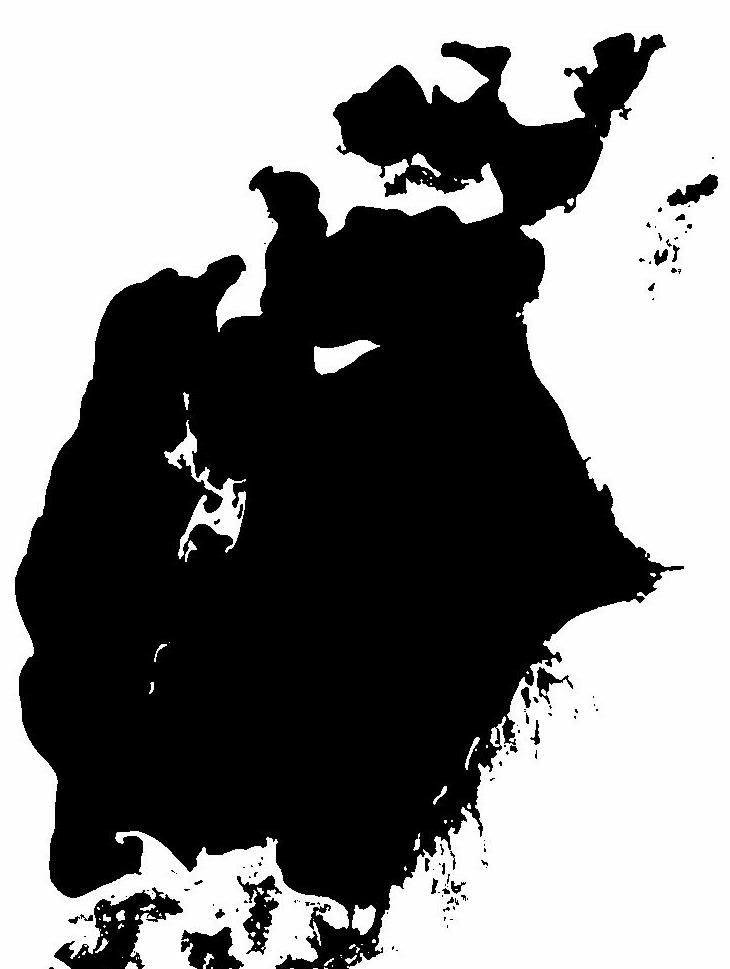
\includegraphics[width=\textwidth]{../img/1977w.jpg}
        \caption{1977}
    \end{subfigure}
    \begin{subfigure}[b]{0.19\textwidth}
        \centering
        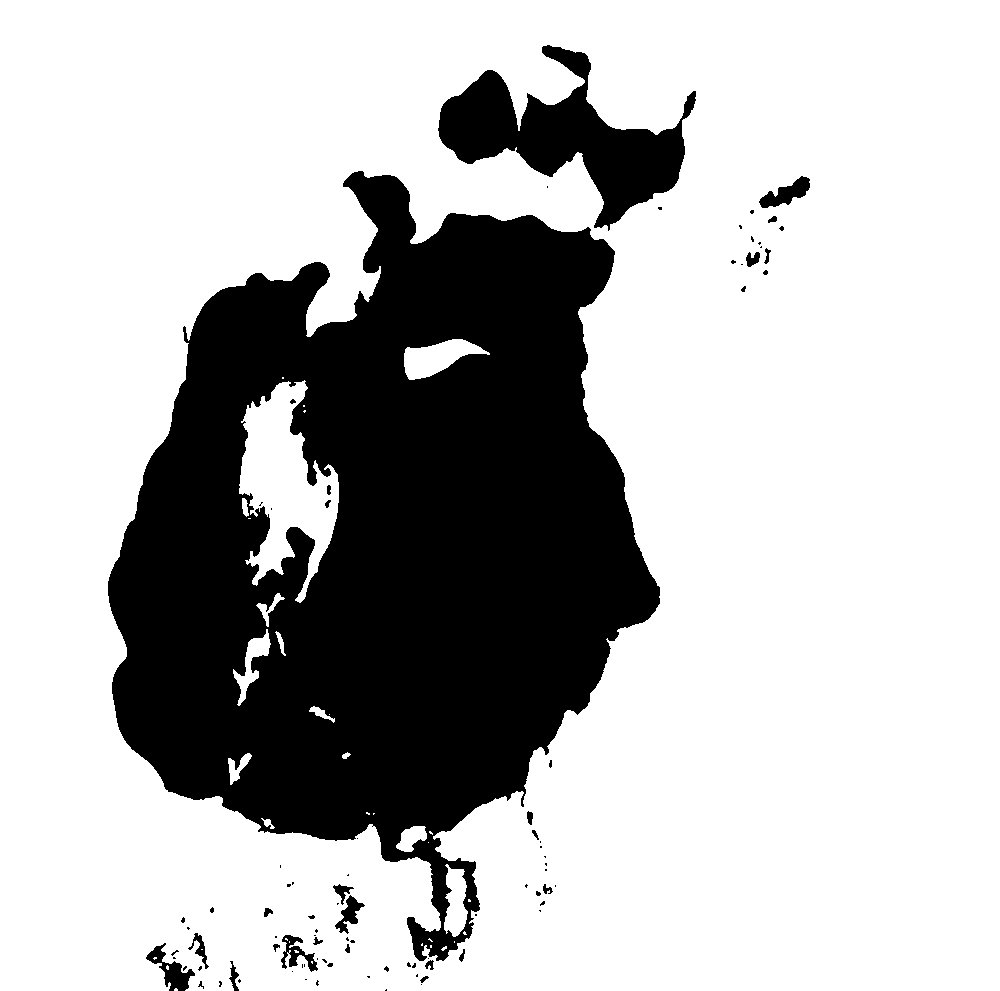
\includegraphics[width=\textwidth]{../img/1987w.jpg}
        \caption{1987}
    \end{subfigure}
    \begin{subfigure}[b]{0.19\textwidth}
        \centering
        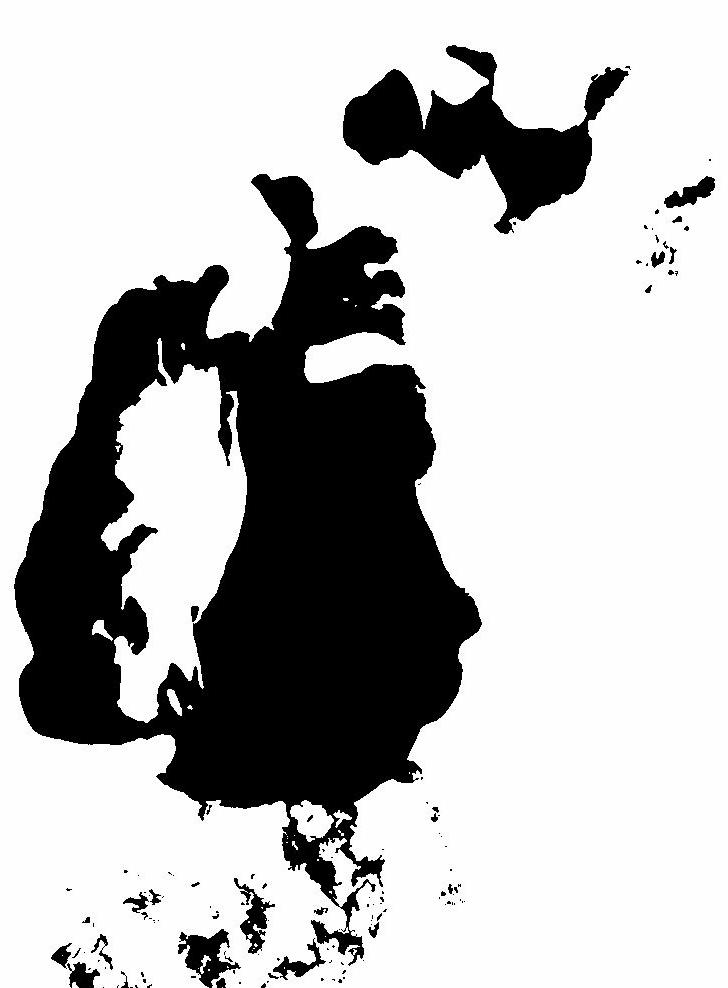
\includegraphics[width=\textwidth]{../img/1998w.jpg}
        \caption{1998}
    \end{subfigure}
    \begin{subfigure}[b]{0.19\textwidth}
        \centering
        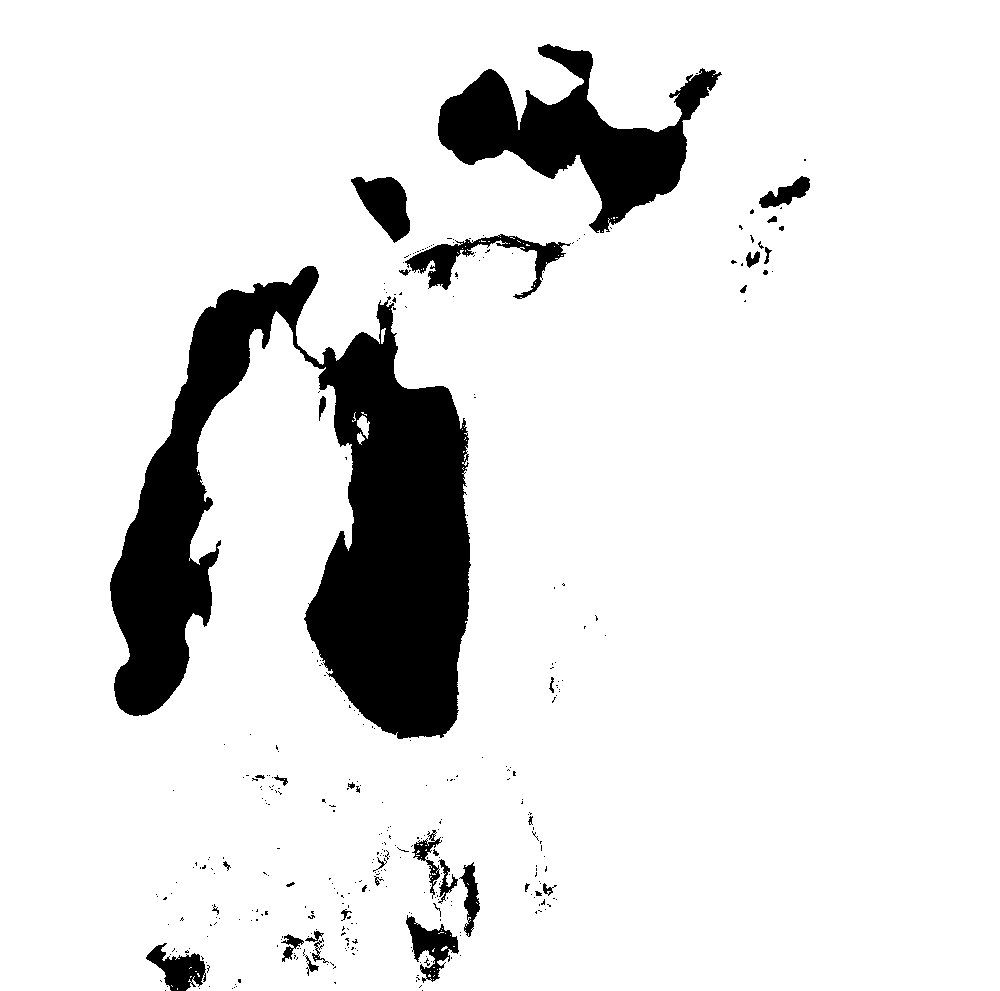
\includegraphics[width=\textwidth]{../img/2006w.jpg}
        \caption{2006}
    \end{subfigure}
    \begin{subfigure}[b]{0.19\textwidth}
        \centering
        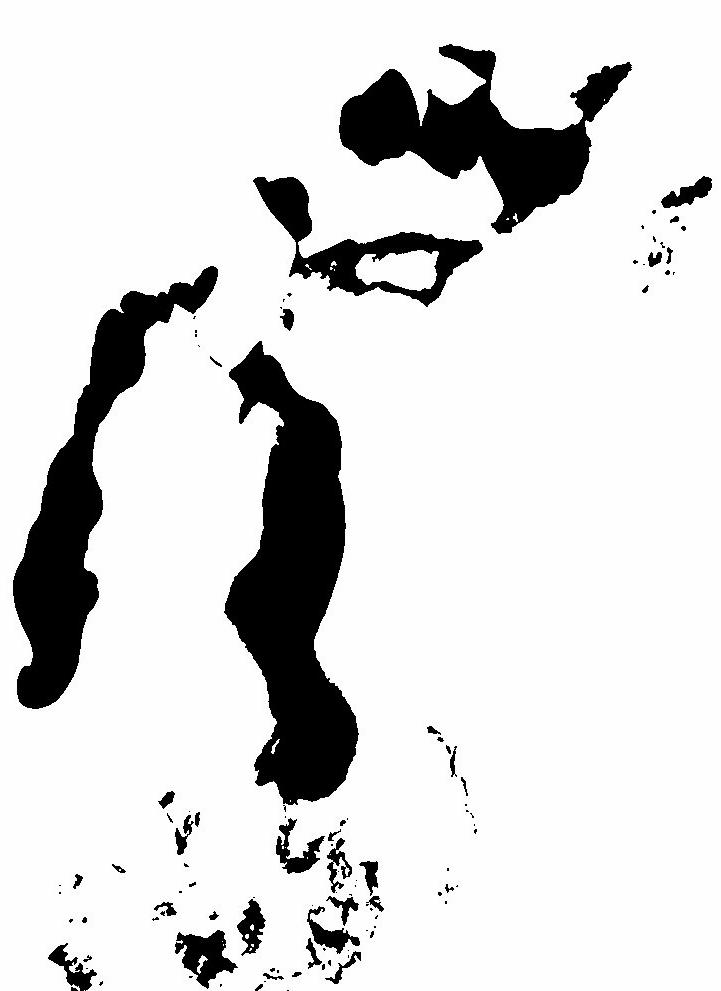
\includegraphics[width=\textwidth]{../img/2010w.jpg}
        \caption{2010}
    \end{subfigure}
    \begin{subfigure}[b]{0.19\textwidth}
        \centering
        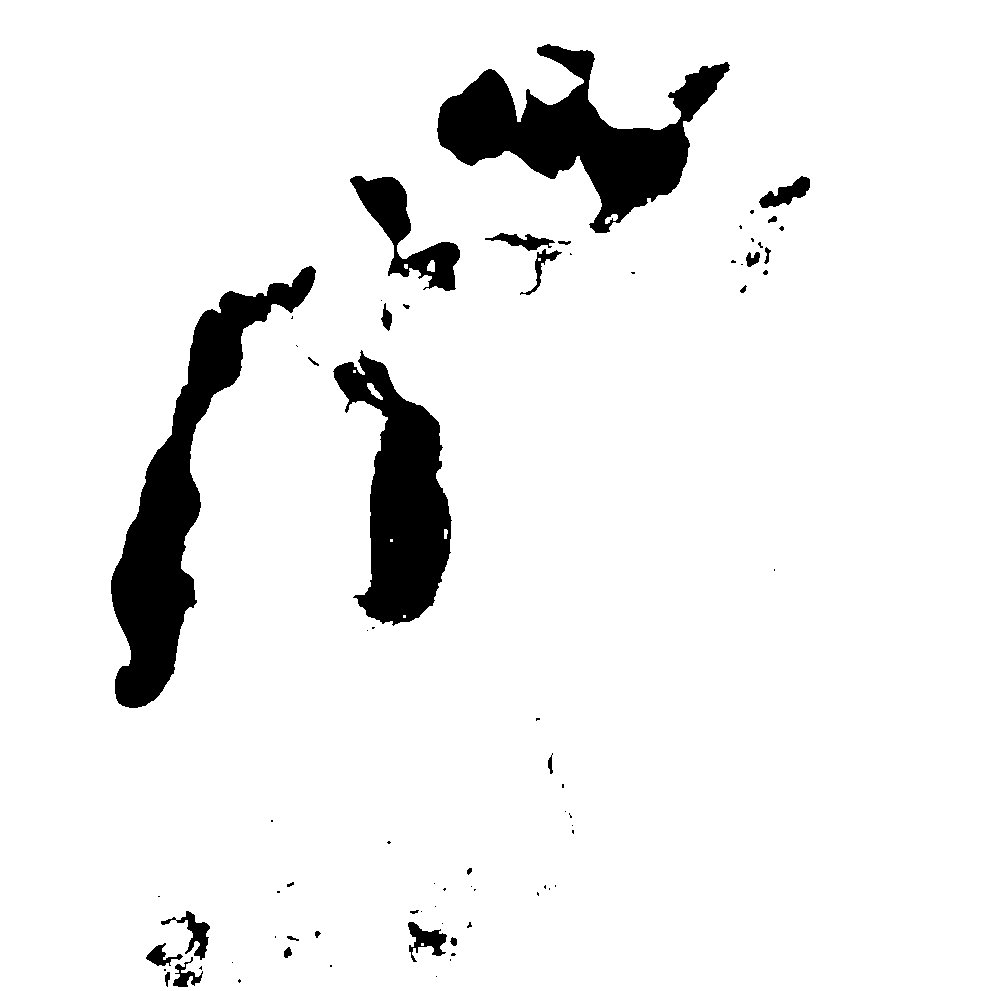
\includegraphics[width=\textwidth]{../img/2013w.jpg}
        \caption{2013}
    \end{subfigure}
    \begin{subfigure}[b]{0.19\textwidth}
        \centering
        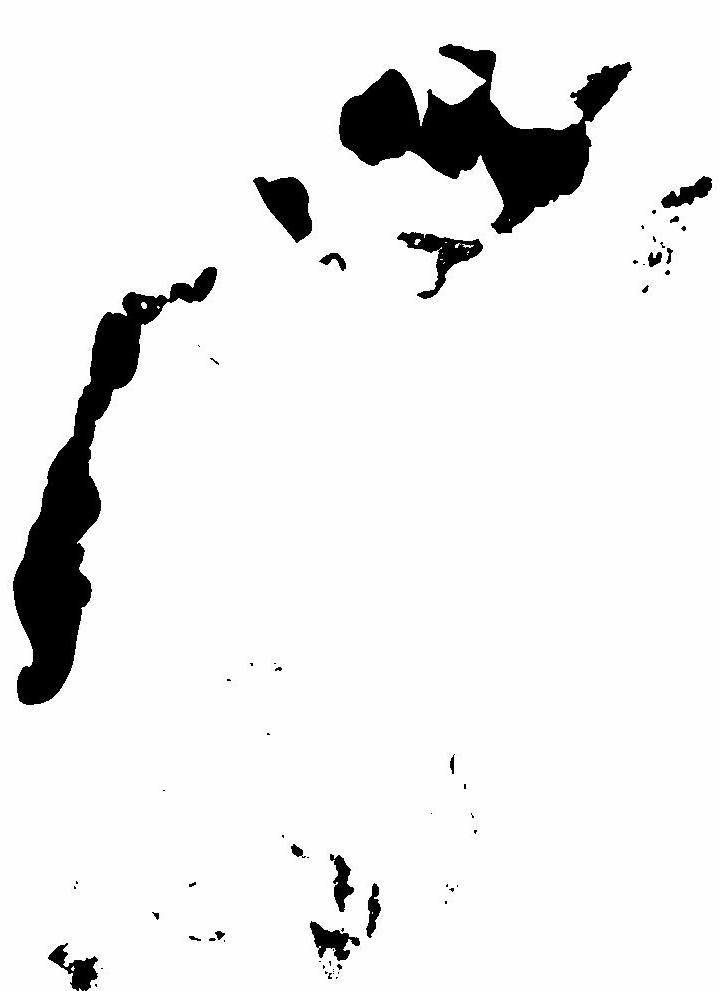
\includegraphics[width=\textwidth]{../img/2014w.jpg}
        \caption{2014}
    \end{subfigure}
    \begin{subfigure}[b]{0.19\textwidth}
        \centering
        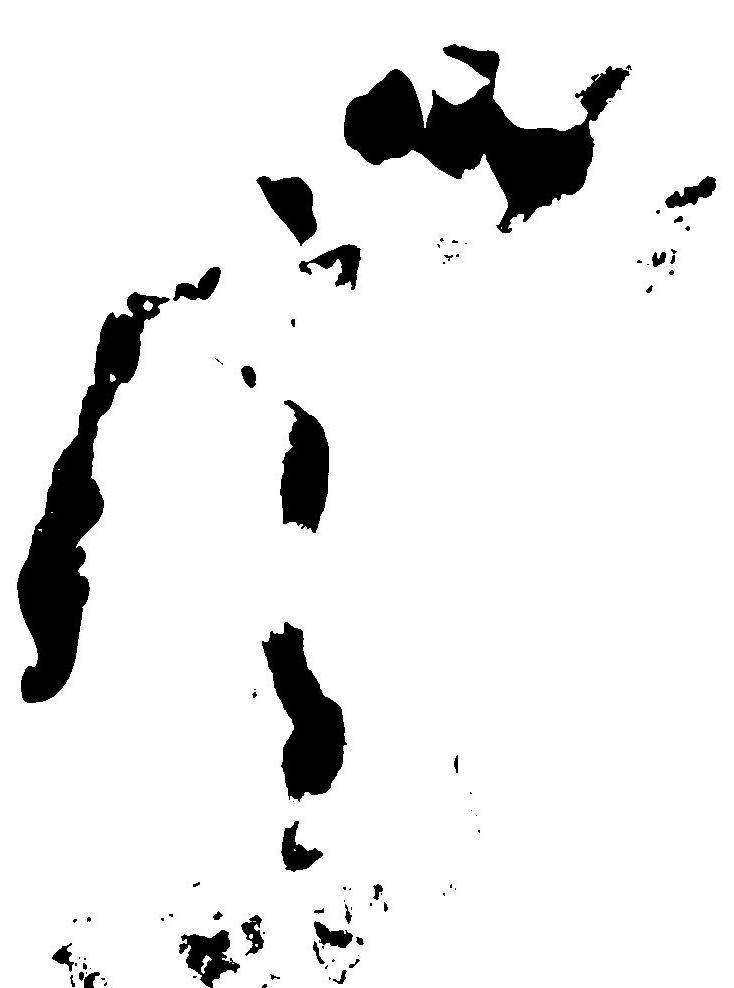
\includegraphics[width=\textwidth]{../img/2015w.jpg}
        \caption{2015}
    \end{subfigure}
    \begin{subfigure}[b]{0.19\textwidth}
        \centering
        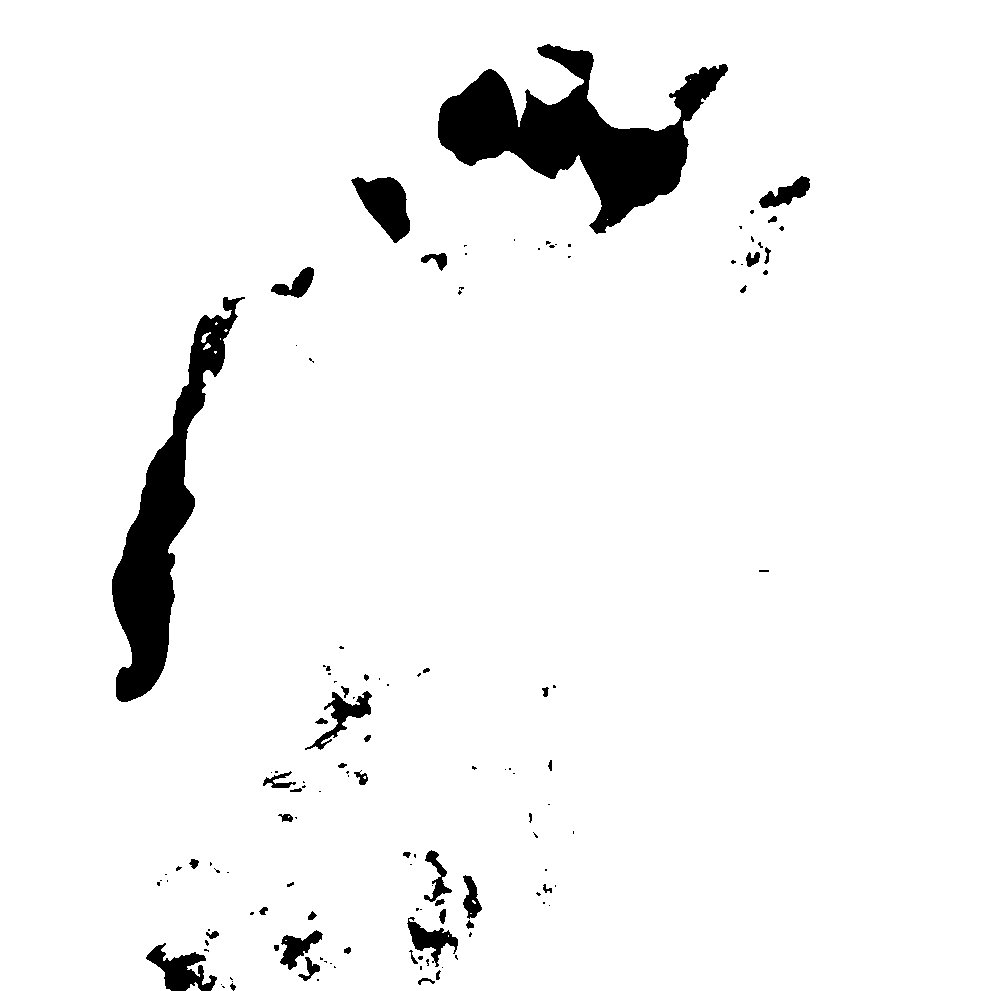
\includegraphics[width=\textwidth]{../img/2019w.jpg}
        \caption{2019}
    \end{subfigure}
    \begin{subfigure}[b]{0.19\textwidth}
        \centering
        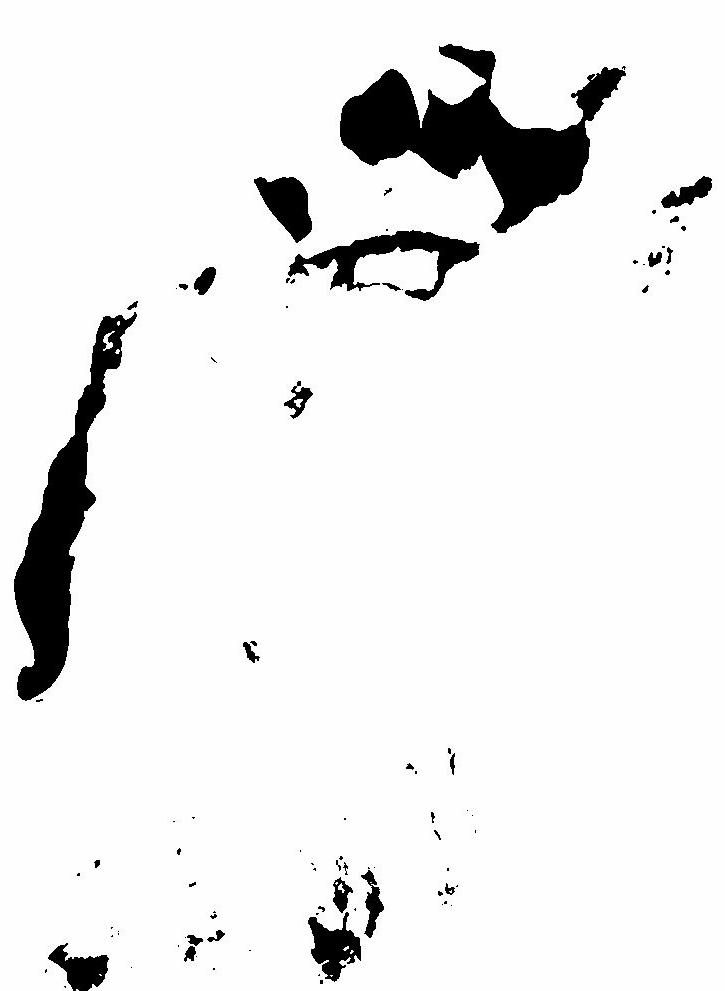
\includegraphics[width=\textwidth]{../img/2021w.jpg}
        \caption{2021}
    \end{subfigure}
    \caption{\emph{Processed images of the Aral Sea.
            In particular, they are the result of a sequence of k-mean clustering, threshold and despeckle.
            All pictures have been taken in a different year.}}
    \label{fig:appendixsurface}
\end{figure}

\begin{figure}[H]
    \centering
    \begin{subfigure}[b]{0.19\textwidth}
        \centering
        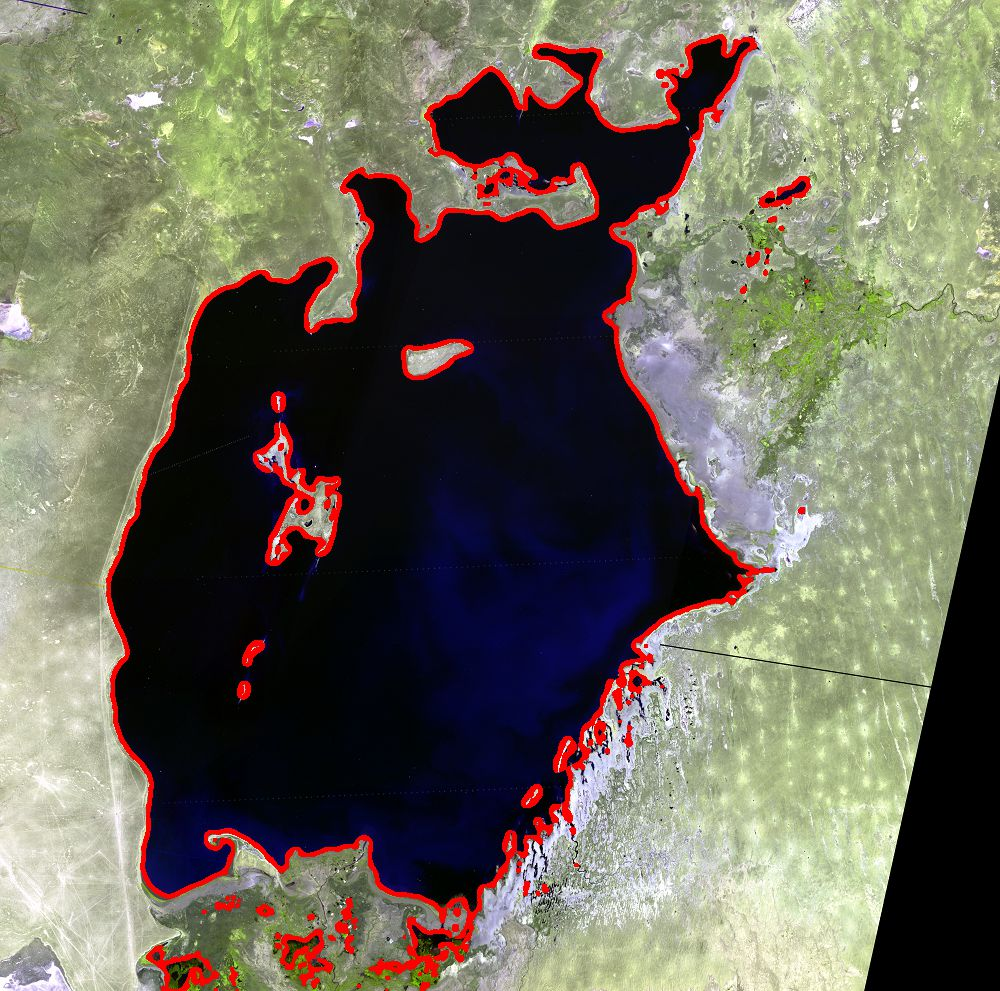
\includegraphics[width=\textwidth]{../img/1977o.jpg}
        \caption{1977}
    \end{subfigure}
    \begin{subfigure}[b]{0.19\textwidth}
        \centering
        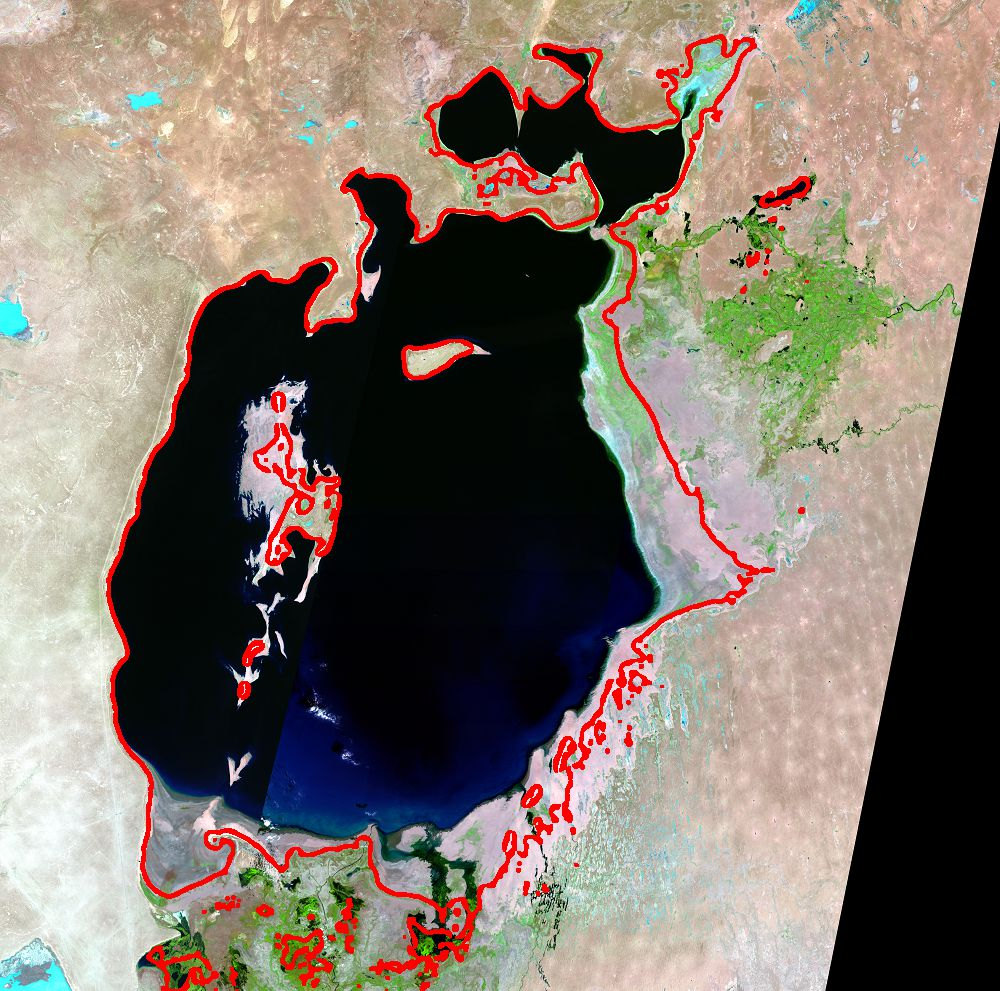
\includegraphics[width=\textwidth]{../img/1987o.jpg}
        \caption{1987}
    \end{subfigure}
    \begin{subfigure}[b]{0.19\textwidth}
        \centering
        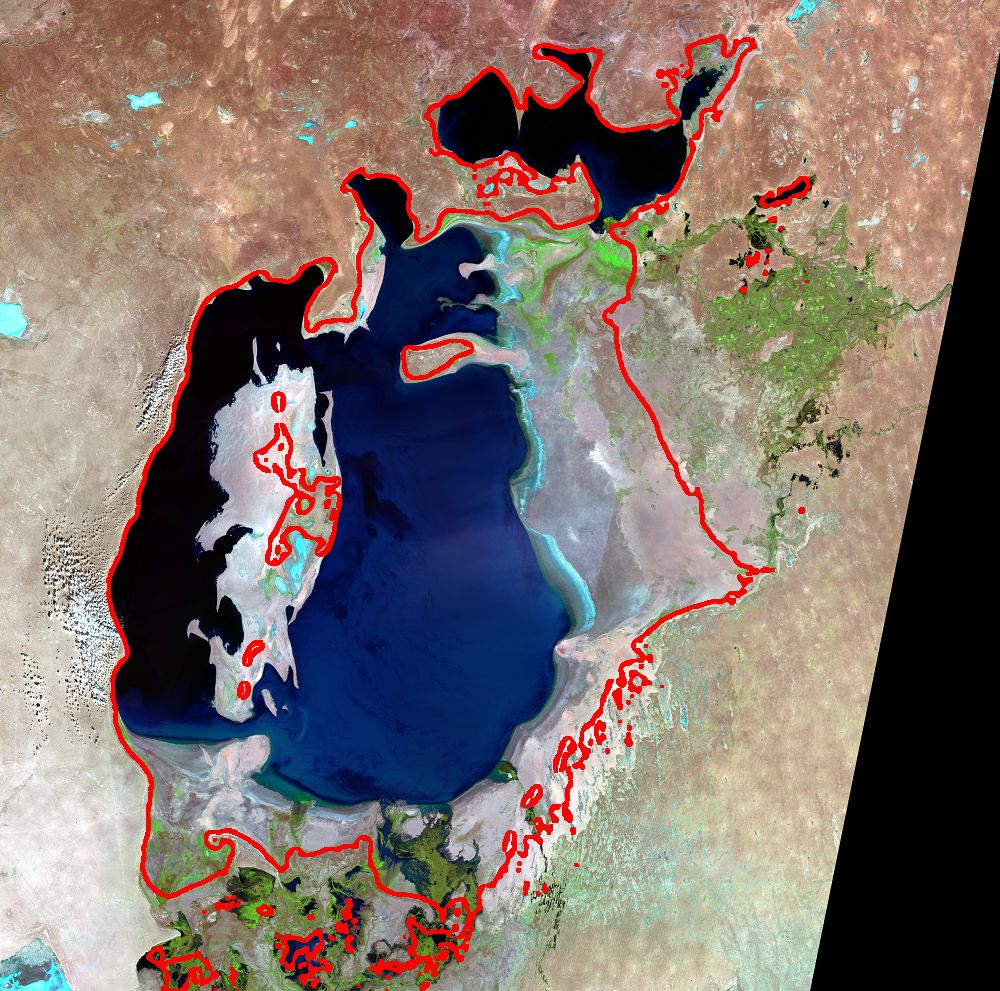
\includegraphics[width=\textwidth]{../img/1998o.jpg}
        \caption{1998}
    \end{subfigure}
    \begin{subfigure}[b]{0.19\textwidth}
        \centering
        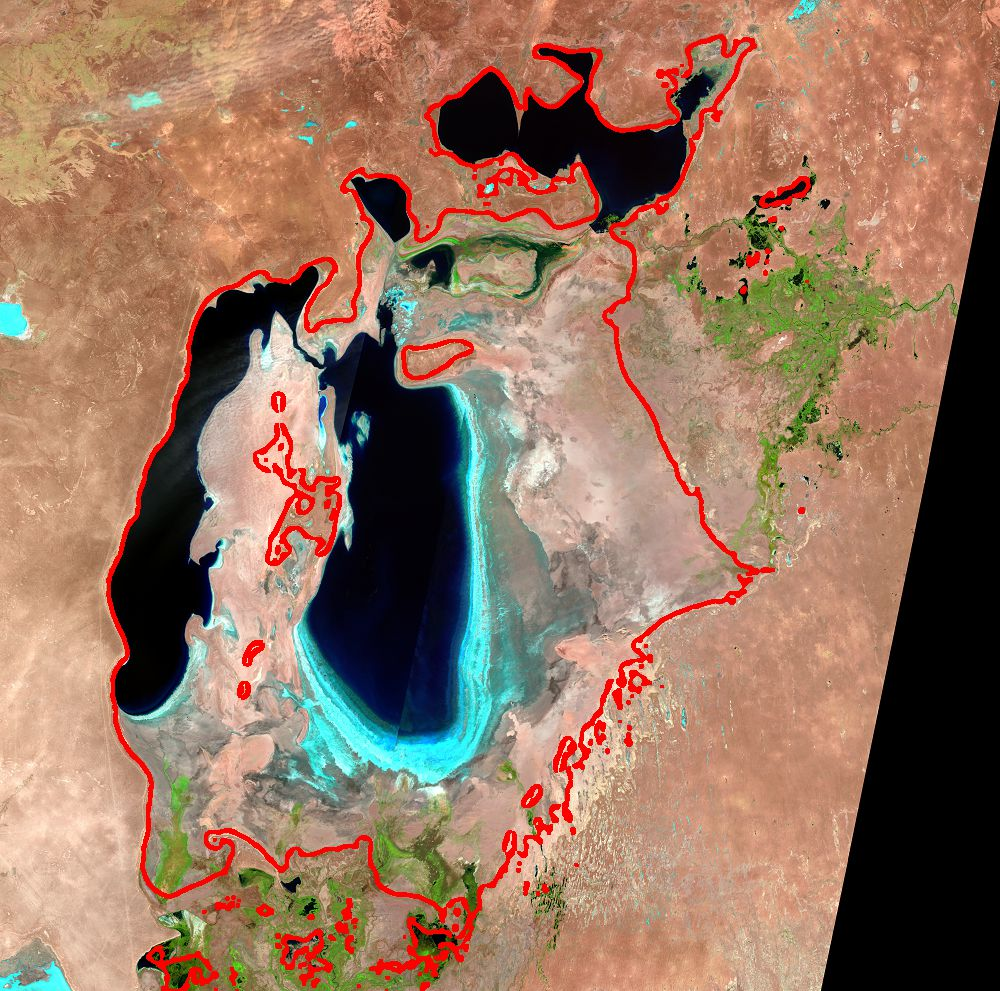
\includegraphics[width=\textwidth]{../img/2006o.jpg}
        \caption{2006}
    \end{subfigure}
    \begin{subfigure}[b]{0.19\textwidth}
        \centering
        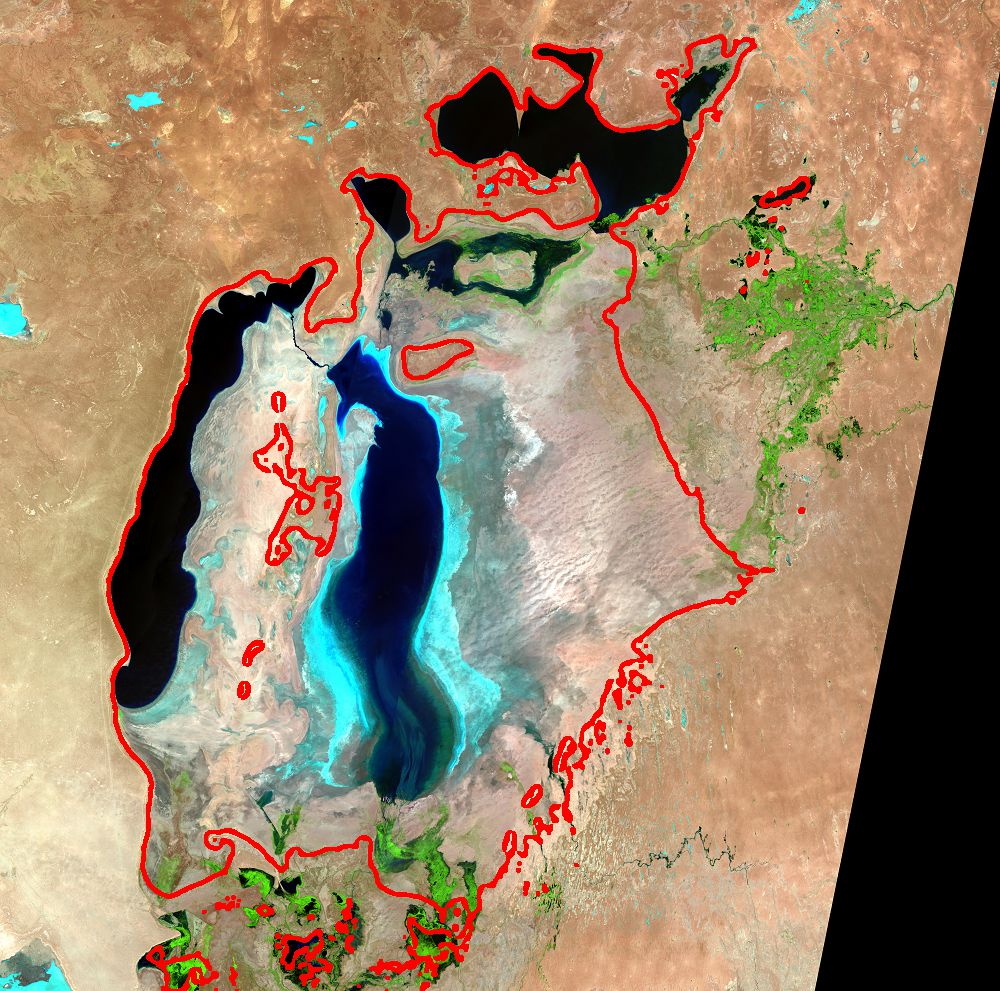
\includegraphics[width=\textwidth]{../img/2010o.jpg}
        \caption{2010}
    \end{subfigure}
    \begin{subfigure}[b]{0.19\textwidth}
        \centering
        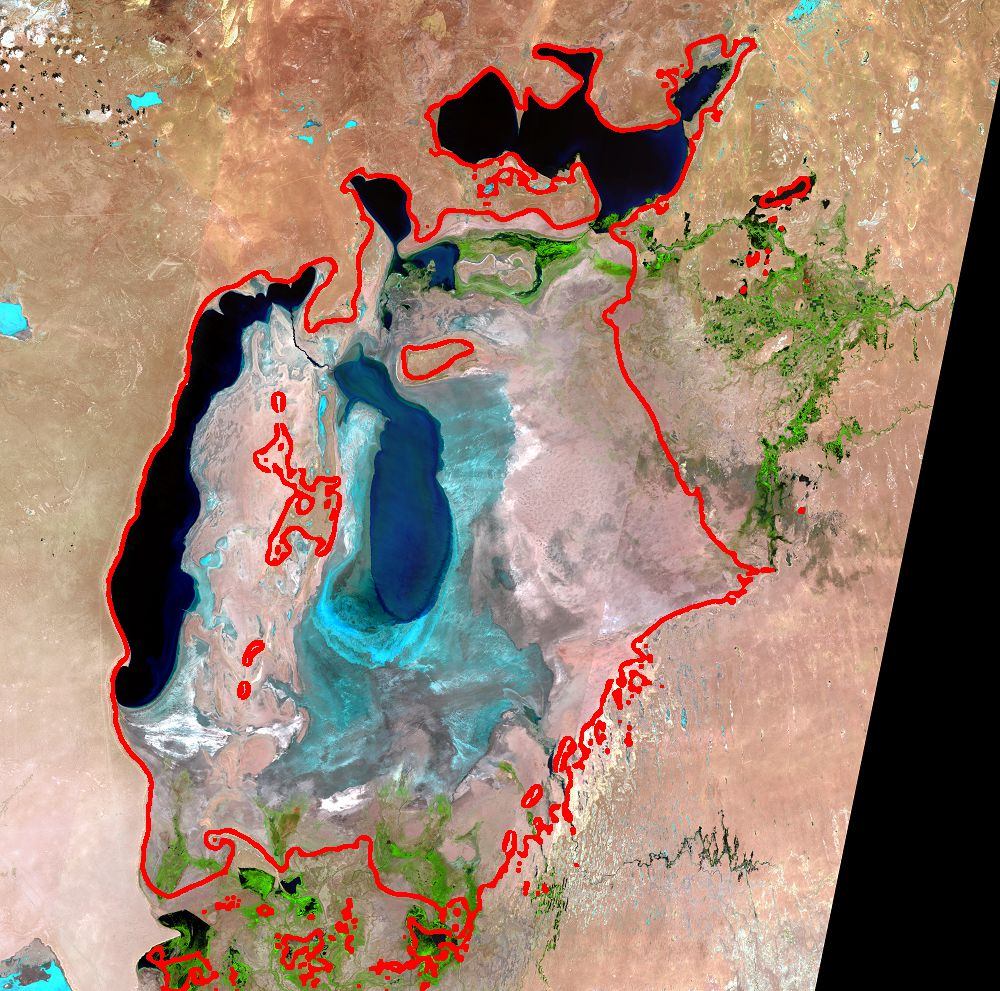
\includegraphics[width=\textwidth]{../img/2013o.jpg}
        \caption{2013}
    \end{subfigure}
    \begin{subfigure}[b]{0.19\textwidth}
        \centering
        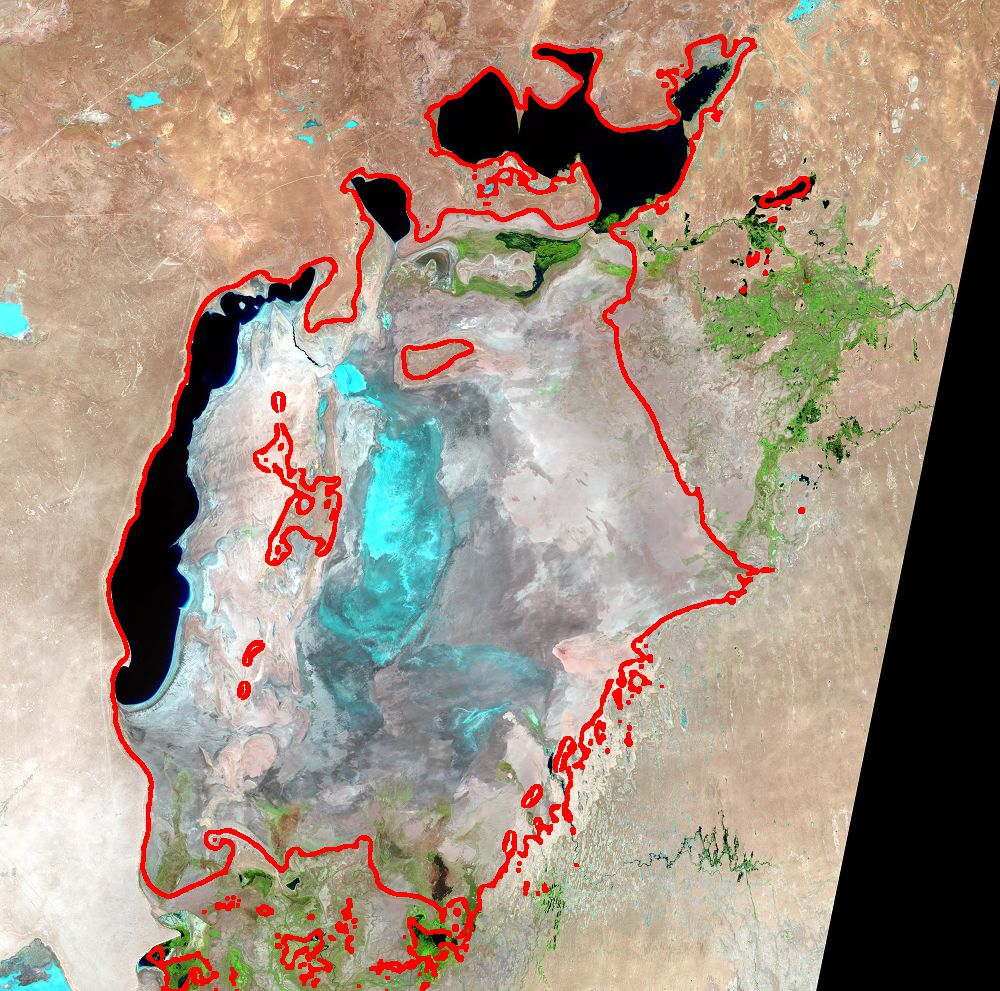
\includegraphics[width=\textwidth]{../img/2014o.jpg}
        \caption{2014}
    \end{subfigure}
    \begin{subfigure}[b]{0.19\textwidth}
        \centering
        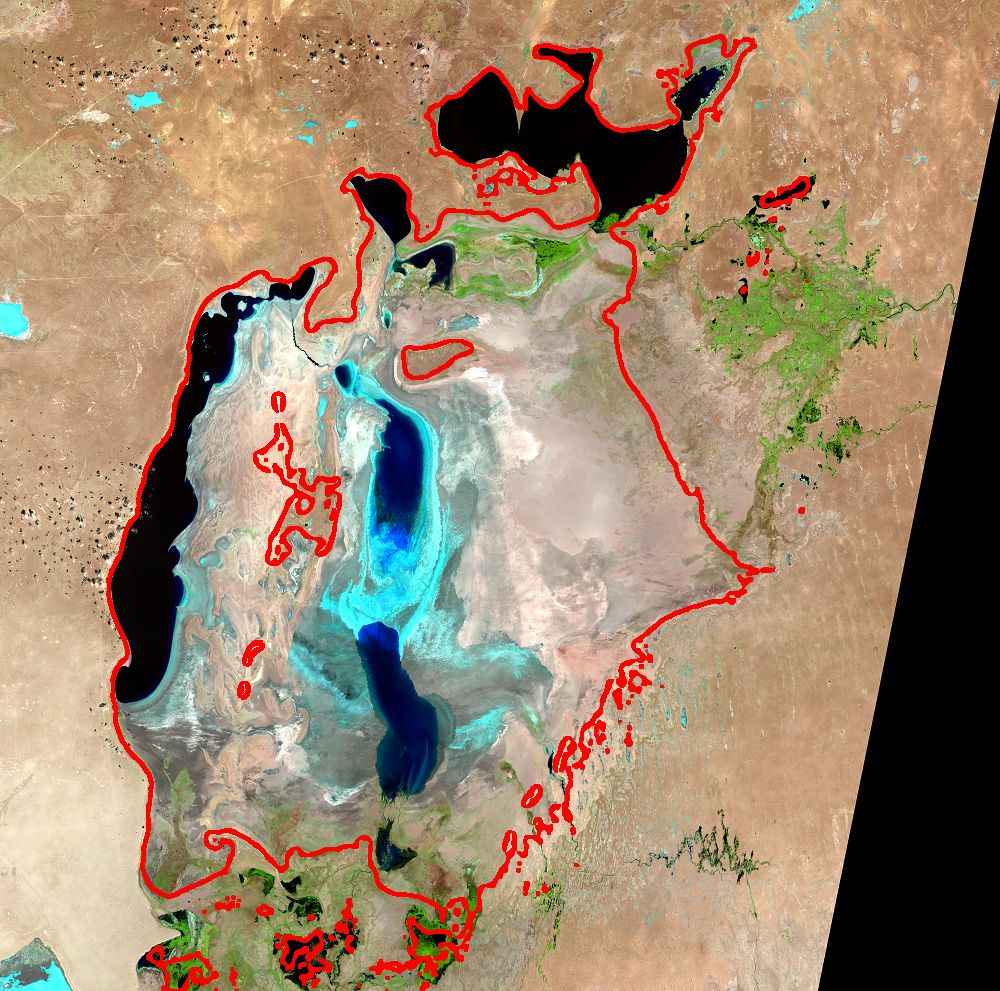
\includegraphics[width=\textwidth]{../img/2015o.jpg}
        \caption{2015}
    \end{subfigure}
    \begin{subfigure}[b]{0.19\textwidth}
        \centering
        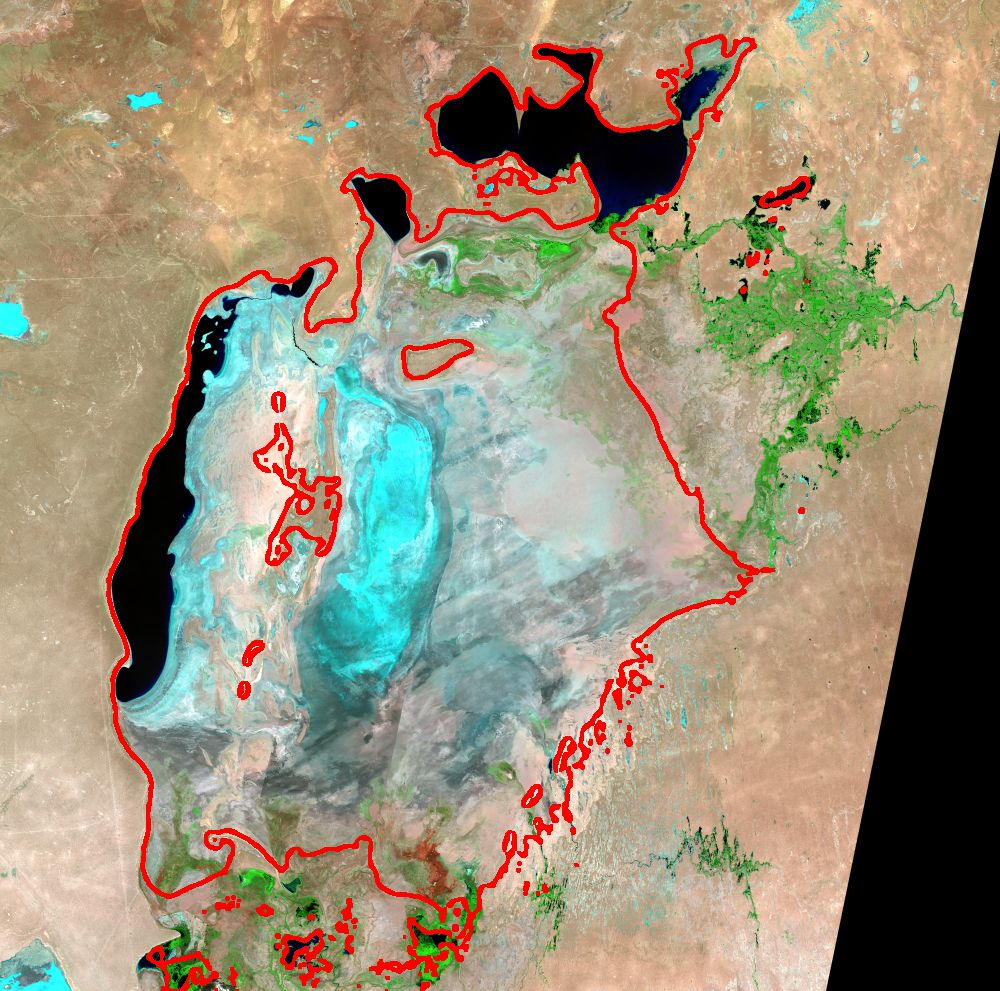
\includegraphics[width=\textwidth]{../img/2019o.jpg}
        \caption{2019}
    \end{subfigure}
    \begin{subfigure}[b]{0.19\textwidth}
        \centering
        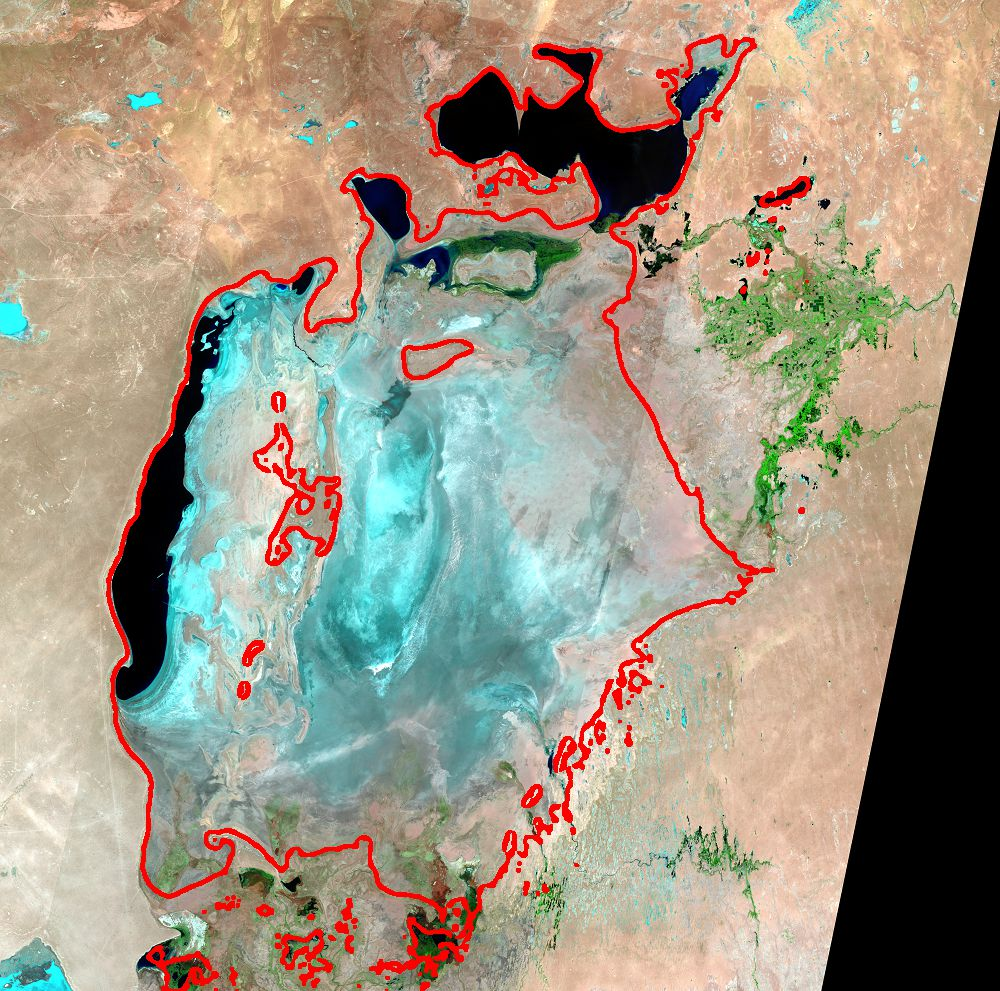
\includegraphics[width=\textwidth]{../img/2021o.jpg}
        \caption{2021}
    \end{subfigure}
    \caption{\emph{Processed images of the Aral Sea.
            In particular, they are the result of the transparent zero command executed between the original images and the colored edges.
            All pictures have been taken in a different year.}}
    \label{fig:appendixedges}
\end{figure}

\printbibliography

\end{document}
